\documentclass[12pt]{article}
%\usepackage{tocloft}% to configure the ToC <<<<<
%\setlength{\cftsecnumwidth}{4.5ex}% set the width to the section number in the ToC <<<<<
%\renewcommand{\thesection}{\Roman{section}.} 
%\renewcommand{\thesubsection}{\quad \Alph{subsection}.}
%\renewcommand{\thesubsubsection}{\qquad \roman{subsubsection}.}

\usepackage{amssymb,amsmath,amsfonts,bbm,bm,dcolumn,booktabs,eurosym,geometry,ulem,graphicx,color,xcolor,setspace,sectsty,comment,float,caption,pdflscape,subfigure,array,hyperref,listings}
\usepackage{xurl}
\usepackage[font=bf]{caption}
\usepackage[bottom]{footmisc}

\lstset{
basicstyle=\small\ttfamily,
columns=flexible,
breaklines=true
}

\hypersetup{
    colorlinks,
    linkcolor={black},
    citecolor={blue!35!black},
    urlcolor={blue!35!black}
}
\normalem
\interfootnotelinepenalty=10000
\setcounter{tocdepth}{2}

\geometry{left=1.0in,right=1.0in,top=1.0in,bottom=1.0in}
\usepackage[style=authoryear,backend=bibtex,maxcitenames=2]{biblatex}
\addbibresource{biblio.bib}

\begin{document}
\title{Predicting Intraday Trading Volume with News Sentiment: An Analysis of U.S. Airline Stocks}
\author{Steven VanOmmeren\thanks{\href{mailto:sevanommeren@gmail.com}{sevanommeren@gmail.com}. A complete replication package of this project is available at \url{https://github.com/svanomm/svo-directed-practicum}. Analysis datasets are available upon request.}}
\date{\today}
\maketitle
\begin{abstract}
\noindent
    When institutional traders buy or sell large amounts of stock, they often have to consider the impact of their trades on the market price. Existing literature has shown that trading volume can be reliably forecasted and can translate to reduced price impact on large trades. In this paper, we attempt to model 15-minute ahead trading volume for 7 major U.S. airlines with a large set of financial variables as well as sentiment measures from the Global Database of Events, Language, and Tone (GDELT). Through a combination of feature engineering, model selection, and hyperparameter tuning, we achieve an out-of-sample $R^2$ of just over 70\% in the prediction of 15-minute-ahead trading volume, over a testing period of approximately 18 months. Our best model explains 25\% more variation than a naive forecast, and is comparable with state-of-the-art models in the literature. We find that sentiment measures improve the model's predictions, but only marginally. These results suggest that sentiment measures are not necessary for accurate trading volume prediction, but they do not hurt the model's performance either. 
\end{abstract}
\newpage
\tableofcontents
\newpage

\doublespacing
\section{Introduction}
The commercial airline industry is somewhat unique in that information about adverse events streams nearly 24/7/365, is highly publicized, and has potential to dramatically affect public trust in the company. In today's digital world, news of a fatal plane crash typically appears online within an hour. Knowledge of a plane crash or other adverse event could significantly impact the airline's stock, either because the event reveals additional information to the public or because traders think that the event will matter. In addition, the general lack of after-hours trading for U.S. commercial airline stock allows real-time news sentiment to anticipate stock market movements.

We examine the impact of such events on airline stock volume at the near-real-time level. Specifically, we leverage data from the Global Database of Events, Language, and Tone (GDELT) (\textcite{leetaru2013gdelt}) to scrape a rich set of sentiment measures from 1.3 million news articles mentioning the major U.S. commercial airlines. We additionally use a large language model to encode additional sentiment from the headline of the GDELT articles. We use these (and other) data to predict intraday trading volumes for 7 major U.S. airline stocks in 15-minute increments during the trading days from January 2018 to May 2025.

This paper appears to be the first to publicly examine such a large volume of real-time GDELT data, the first to examine the effects of news sentiment on stock volumes at a sub-daily level in the airline industry, and the first to consider the large set of supplemental sentiment indicators offered by GDELT for stock prediction. All of our code used to scrape and examine GDELT is available free and open-source. The focus of this paper is on the problem of forecasting trading volume; we leave an assessment the actual profitability of our models to future work.

The rest of this paper is as follows: the following section reviews the relevant literature on stock volume prediction, sentiment analysis, and the use of GDELT data. Section \ref{section:methods} describes the data preparation and modeling techniques used in this paper. Section \ref{section:results} presents the results of our models and other analyses. Section \ref{section:discussion} discusses the implications of our findings and their relation to the existing literature. Section \ref{section:conclusion} concludes.

\section{Literature Review}
\label{section:litreview}

\subsection{Stock Volume Prediction}
The fact that most traders are concerned with predicting stock prices makes stock prices nearly impossible to predict. One consequence of a relatively efficient stock market is that, if a trader discovers an exploitable pattern, the act of trading on that pattern will eventually eliminate its profitability, an idea that \textcite{timmermann2004efficient} call the ``self-destruction of predictability.'' Trading volumes do not provide direct price information, and so they are not subject to the same competition as with prices. As a result, trading volume is highly predictable with the right model, and the literature shows that accurate volume forecasts can provide indirect value to institutional traders by reducing the effective cost of trading.

\textcite{goyenko2024trading} model the potential benefits associated with accurate predictions of trading volume. The authors explain that while trading volume is not particularly useful to a day trader, inaccurate forecasts of volume could lead a large trading firm to miscalculate the price impact of a trade. In the authors' theoretical model, overestimating the amount of trading volume when making a large trade increases the net trading cost to the firm. Specifically, price impact is assumed to be proportional to the trade's share of total volume:
\begin{equation}
    |Price Impact_{t}| = \alpha\frac{v_{t}}{V_{t}}, \qquad 0< \alpha < 1,
\end{equation}
where $v_{t}$ is the volume of a given trade, and $V_{t}$ is the total volume of all trades at time $t$. The result is that buying (or selling) a large proportion of total volume makes the trade more costly, because price is higher (or lower) than it would be otherwise. The authors create a predictive model of changes in the log of dollar trading volume using technical indicators for 4700 stocks over a period of 1258 days. Their best model (an LSTM with 175 features) obtains an $R^2$ of around 20\% relative to the prediction accuracy of a moving average model. This demonstrates that, unlike stock price prediction, models can consistently predict daily trading volumes over a wide range of stocks. The authors then translate their volume predictions into simulated trading strategies, finding a significant net-of-cost return.

\textcite{cucuringu2025forecasting} investigate the ability of machine learning models to predict intraday trading volumes. The authors analyze 15-minute data over a period of 6 months for each constituent stock in the S\&P 500 index. A baseline model is able to predict out-of-sample volumes with an $R^2$ of 0.265, while their best model attains an $R^2$ of 0.624. The authors then demonstrate the usefulness of their model for large traders seeking to minimize the price impact of a trade. Their model improves the volume-weighted average price (VWAP) order execution risk for a sample of 5 stocks by an average of around 29\%, compared to a baseline model.

\textcite{satish2014predicting} make the case for using a statistical model to predict trading volumes. The authors explain that at the time,  the typical approach taken by firms was to just use moving averages of trading volumes as a predictor. The authors combine two ARMA models with varying levels of historical data (intraday and daily) to predict trading volume. After calibrating their model, the authors were able to increase VWAP error performance by 9\% compared to the typical moving average approach. Notably, the authors explain that news events can affect VWAP tracking error, though they do not include news sentiment in their model.

\subsection{Sentiment Analysis}
Sentiment analysis can generally be defined as the extraction of meaningful (and preferably quantifiable) information from a piece of text. A full review of the applications of sentiment analysis is far beyond the scope of this paper.\footnote{For further reading, see \textcite{mejova2009sentiment} and \textcite{wankhade2022survey}.} However, we discuss some usecases of sentiment analysis as they relate to our paper, which is extracting information content from news articles for forecasting purposes.

We provide a basic motivation for the use of financial sentiment analysis.\footnote{Additional motivation with a more economic-theoretic underpinning can be found in \textcite{kaplanski2010sentiment}.} A company's perceived value can change over time when events reveal additional information about the company to the public. For example, an unexpected natural disaster could destroy some of the company's assets, devaluing its business. Another example would be a company's product experiencing sudden failure (e.g. a plane malfunction), which reveals additional information about the quality of the company's products. In both cases, even if a person's perception of the company remains unchanged, they may believe that other people have changed their perception of the company. As a result, we can expect an increased trading volume of the company's stock, as people adjust their holdings to align with their new beliefs about the company. People find out about such events by reading news articles, and so it is natural to extract sentiment from popular news articles to anticipate how relevant events will be perceived by the public. 

There are many ways to evaluate the sentiment of a piece of text. The most basic and common approach is to classify text as having a positive (i.e. good) or negative (bad) sentiment, also called ``tone.'' Another basic and commonly-seen sentiment measure is to count the number of words or articles discussing a particular topic. In the context of news articles, a spike in the number of articles mentioning an airline company likely indicates that something important has happened, which could affect its stock. While basic measures often capture a large portion of the sentiment from a news article, there are many ways to measure positive/negative tone, as well as more nuanced dimensions of sentiment. Additional basic measures include: counting the number of positive/negative-sentiment words in the text, or assessing the relation of positive to negative words (i.e. polarity or dispersion).

\textcite{kaplanski2010sentiment} study the effects of aviation disasters on the overall stock market. While a large-scale aviation disaster would expectedly affect aviation stocks, the authors hypothesize that the overall stock market could also be affected by a general sense of anxiety or increased aversion to risk. Analyzing the excess market returns surrounding 288 aviation disasters over a period of 58 years, the authors show that the first day following a plane crash sees decreased rates of return in the market, with the abnormal returns recovering over a period of about 2 weeks. The market-wide decrease results in losses that are on average over 60 times larger than the direct economic loss of the disaster itself. The authors interpret these results as evidence of the psychological effect of anxiety-inducing media coverage.

\textcite{loughran2011liability} analyze SEC filings to identify words that indicate financial sentiment for businesses. The authors identify various sentiment dimensions of interest: positive (i.e. good news), negative, uncertainty, litigiousness, and strong/weak modalities. After identifying words that fit into these dimensions, one can assess the sentiment of a financial form by counting how often the words appear in the text. The major contribution of this work is in recognizing that sentiment measures should be specific to the domain of interest, and in providing measures that identify financial sentiment in particular.

While sentiment analysis has historically relied on identifying specific words and counting their occurrences in a document, recent advances in machine learning have allowed for more sophisticated approaches. Large language models (LLMs) encode text into a high-dimensional vector space to capture more complex relationships between words in an article. LLMs have become a popular addition to sentiment analysis. \textcite{huang2023finbert} introduce FinBERT, a large language model specifically designed for extracting information from financial text. The authors trained an existing LLM architecture on financial filings, analyst reports, and earnings call transcripts, with the goal of predicting positive/negative sentiment of the document. They find that FinBERT outperforms more traditional sentiment measures.

\subsection{GDELT}
Previous studies have assessed the usefulness of GDELT for predicting stock prices. However, apparently all of them have aggregated GDELT to a daily level, rather than using it at its original real-time 15-minute increments. To our knowledge, only one study has taken advantage of the GDELT sentiment measures outside of the basic metrics of tone, count of articles, and number of positive/negative sentiment words for predicting financial markets.

\textcite{nashir2023indonesian} incorporate GDELT data into a machine learning model to predict stock prices. The authors source a long span of daily stock data from Jan. 2008 to Dec. 2022 (5479 observations), specifically for the Jakarta Stock Exchange (JKSE) index of Indonesian stocks. The authors study 4 sentiment measures using GDELT data: tone, optimism, attention, and tone dispersion. These metrics are calculated at the daily level. The authors then train a modified version of an LSTM model using time series cross-validation. The authors document an extensive hyperparameter optimization, which yielded an improved model with a mean absolute percentage error (MAPE) of 0.8\%. They additionally find that a model trained with only the ``optimism" feature slightly outperforms the model with all four sentiment measures.\footnote{The combined model outperforms the other models that include only a single sentiment metric (tone, attention, or tone dispersion).} The authors do not compare their results to a Naive forecast.

\textcite{wang2024ensemble} use GDELT data to inform the prediction of a variety of individual stocks and indices. They do not identify articles specific to each stock, instead summing the number of article mentions and the sum of tone for each CAMEO code. CAMEO codes provide high-level descriptions of conflict identified in an article, e.g. ``Threaten" or ``Engage in political dissent." The authors then evaluate causal relationships between the CAMEO-specific metrics with each stock price at the daily level from Jan. 2018 to Feb. 2022. These causal relationships are incorporated into an LSTM model to predict stock prices. The authors report that this model performs best out of a variety of other models (including ARIMA, VAR, etc.). Unfortunately, the authors do not compare the performance of their model to a Naive prediction, and a close look at their predicted vs actual charts shows that their best model essentially predicts the previous stock price. In other words, they likely do not beat a Naive forecast.

\textcite{consoli2021information} assess the use of GDELT for modeling sovereign spreads in the European bond market. The time series of interest is the sovereign spread of Italy vs Germany with respect to 10-year bond yields, with 468 data points covering a time period of Mar. 2015 to Aug. 2019. The authors filtered GDELT to identify articles specific to macroeconomic discussions in the locations of interest. They identify a subset of 45 GDELT variables that are both quantitatively and qualitatively relevant to bond markets. The authors then include these variables along with bond market data in a probabilistic LSTM model, yielding an out-of-sample R-squared of 0.23 for predicting changes in the dependent variable. While the study suffers from a small sample size and does not compare its accuracy to a Naive forecast, it provides robust evidence that GDELT could be useful for predicting bond markets.

\textcite{jakel2019using} investigates correlations between GDELT sentiment and the stock prices of U.S. technology companies. The author sourced approximately 60,000 articles over a 29-day period in 2019. He then averaged the sentiment tone by company and day to join to 29 days of stock price data for Facebook, Apple, Amazon, Alphabet and Tesla. Analyzing the correlation between sentiment and stock price, the author found a generally contrarian relationship. However, the results are inconclusive due to a small sample size.

\textcite{alamro2019predicting} use GDELT's Tone and count of articles per day to predict TASI, a Saudi stock market index. The authors filtered GDELT data to any articles that mention Saudi Arabia, then aggregate the data to the daily level, averaging the Tone metric and counting the number of articles per day. The authors then test a variety of models to predict the index price, finding that an LSTM model performs dramatically better than more traditional forecasting models.\footnote{Unfortunately, the authors do not report the specification of the LSTM model, any scale-independent measures of model fit, any comparisons to a Naive forecast, any tests of whether the sentiment measures add predictive value, nor any graphs of predicted vs actual stock prices. It is therefore unclear whether the authors' LSTM model provides better-than-Naive performance or if the sentiment measures actually improved the fit of the model.}

\section{Methods}
\label{section:methods}

Below, we explain the data preparation and modelling techniques used to evaluate the usefulness of news sentiment for predicting airline stock volume.\footnote{All processing and modelling was performed on a Windows 10 desktop with the following specifications: 128GB of DDR4 RAM, an Nvidia RTX 2070 Super (8GB VRAM), and an AMD Ryzen 5 3600 processor.} The resulting dataset has a row for each stock ticker and 15-minute trading period, and columns for the various financial and sentiment features. The models are trained to predict 15-minute-ahead trading volume for each airline stock.

\subsection{Data Preparation}
\subsubsection{Stocks}
Stock data were downloaded in 15-minute increments during market open from Barchart, for the period Jan. 2018 to May 2025. The following tickers were downloaded:
\begin{itemize}
\singlespacing
    \item AAL: American Airlines Group Inc.
    \item ALGT: Allegiant Travel Company
    \item ALK: Alaska Air Group Inc.
    \item DAL: Delta Air Lines Inc.
    \item JBLU: JetBlue Airways Corp.
    \item LUV: Southwest Airlines Co.
    \item UAL: United Airlines Holdings Inc.
    \item BNO: United States Brent Oil Fund LP
    \item ITA: iShares US Aerospace \& Defense ETF
    \item IYT: iShares US Transportation ETF
    \item JETS: US Global Jets ETF
\end{itemize}
As seen from the list, we include some stocks as control variables that are likely correlated with airline stocks: 3 airplane-related ETFs, and an oil fund.\footnote{Fuel is a major input cost for airlines, and so changes in oil prices can significantly impact airline stocks.} The raw data include the stock's open, high, low, and last price, and volume traded over each 15-minute period. We calculate additional features for each stock:
\begin{itemize}
\singlespacing
    \item High-Low spreads
    \item Last-Open spread
    \item 1-period change in open, high, low, last price, and volume
    \item Change in trading volume compared to same time on previous trading day (10 lags)
    \item 10-period rolling standard deviation of last price
    \item 10-period rolling standard deviation of volume
\end{itemize}
The last 2 measures are meant to capture changes in volatility for a given stock.

We then calculate a variety of moving averages for each metric, with the following windows: 4 periods (1 hour), 8 periods (2 hours), 16 periods (4 hours), and 26 periods (one trading day). For price, volume, change in price, and change in volume, we also calculate 26 periods of 15-minute lags. The data is reshaped so that each observation is a 15-minute bin and stock ticker (for the 7 airline stocks). The features include the stock's own characteristics, as well as the ETFs and oil fund. The final data has 337,795 rows and 800 lagged features for prediction.

We also create indicator variables for each hour of day, day of week, and month of year, as well as indicators for market open and market close. These indicators are meant to capture multilevel seasonality common across the stocks.

\subsubsection{GDELT}
GDELT scrapes news articles from around the world in near-real-time, and provides a rich set of sentiment measures for each article. The data we use is uploaded by GDELT in files every 15 minutes. Each file contains all of the articles that GDELT scraped in a given 15-minute period. We began by programatically downloading files for the approximately 260,000 15-minute periods covering the timeline of 1/1/2018 00:00:00 to 5/30/2025 23:45:00.\footnote{Additional details of our data processing can be found in the Appendix, Section \ref{section:gdelt_details}.} Because we are interested in articles concerning the major U.S. airline stocks, we dynamically filtered the GDELT data during the downloading process. After filtering, 218,574 raw GDELT files were combined for a total of 1,261,785 articles identified.\footnote{The total raw GDELT files kept is less than the theoretical 260,000 files for multiple reasons, including: no airlines mentioned in the past 15 minutes, and sporadic GDELT outages.} We then performed extensive additional cleaning to filter the articles and sentiment measures to those that would likely affect the stock market. After cleaning and filtering, we have 121,655 relevant articles and 118 sentiment measures.

We describe some of the sentiment measures used here, leaving a complete list of the measures for the Appendix, Section \ref{section:gdelt_details}. First is the article's tone, which captures general positive/negative sentiment. We use article count as a proxy for overall attention to the respective airline. 6 of the sentiment measures are finance-specific word counts from \textcite{loughran2011liability}, identifying positive, negative, uncertainty, litigiousness, strong modality, and weak modality words. We use general positive and negative scores from the SentiWordNet 3.0 database (\textcite{baccianella2010sentiwordnet}). The bulk of our sentiment measures count the number of times that specific business-related words are mentioned, such as ``debt," ``inflation," ``money laundering," and many other terms identified by GDELT.

The GDELT data also include each article's headline or title, which we use to extract additional sentiment. Specifically, we use a large language model to embed the article titles in a high-dimensional vector space. Rather than encoding the headlines into a single tone dimension (as in \textcite{huang2023finbert}), we instead use a general-purpose language embedding model and retain 32 dimensions of the embedding space.\footnote{Our chosen model (Qwen3 Embedding 0.6B) embeds text into 1024 dimensions, but we limit to 32 dimensions as a computational constraint and as a form of dimensionality reduction. This model was chosen for its nearly top-ranked performance (at the time of writing) in embedding benchmarks and relatively small size.} These 32 dimensions are then used as additional sentiment measures in the model. Unlike the GDELT sentiment measures, these LLM dimensions have no specific meaning and are in some sense ``black box'' features. However, they may be useful for capturing textual nuances that are not captured by the GDELT measures.

The data at this point is a collection of 121,655 articles with corresponding article-level sentiment measures. To align with the stock data, we need to aggregate the articles into 15-minute bins. Each sentiment measure is aggregated with rolling sums of varying time windows: 1 hour, 4 hours, 12 hours, and 24 hours. Each of these rolling sums is included in the feature set to allow the model to identify combinations of windows that best fit the data. Finally, the data is reshaped so that each observation is a 15-minute-bin and stock ticker. The final data has 750 sentiment features and is joined onto the stock data by time and stock ticker.

\begin{figure}[H]
\centering
\caption{GDELT Data Processing Workflow}
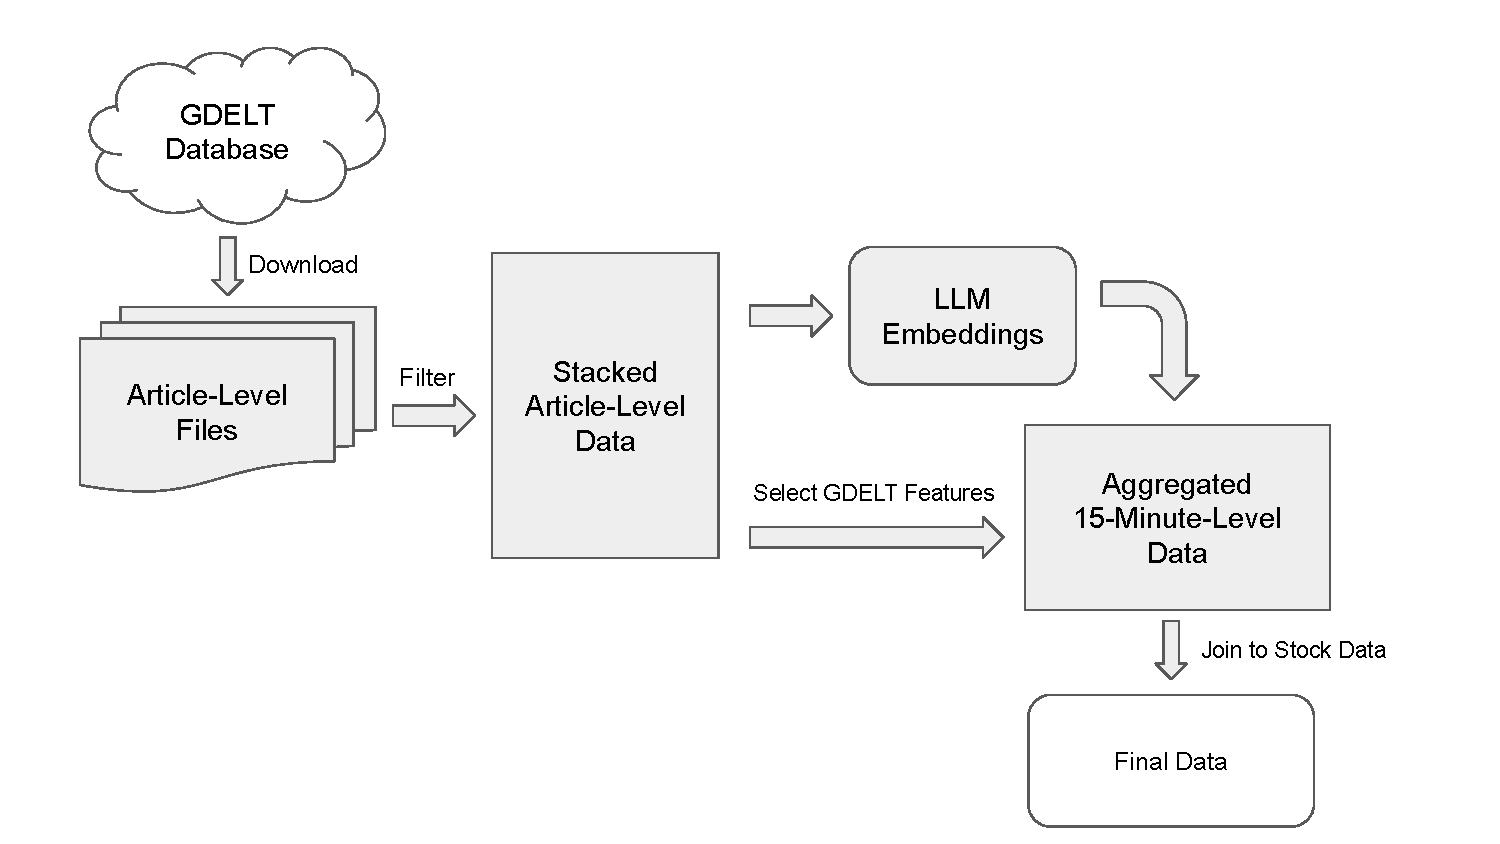
\includegraphics[width=0.8\textwidth]{../Output/GDELT Processing Diagram.pdf}
\end{figure}

\subsection{Modeling}

We test a variety of models on multiple subsets of the features described above to understand which features contribute the most to predicting stock volume. We create the following feature sets:
\begin{itemize}
\singlespacing
    \item \textbf{Time Only}: open/close, hour of day, day of week, and month of year indicators (26 features)
    \item \textbf{Sentiment Only}: 118 GDELT measures, 32 LLM measures, with 1 non-moving average and 4 moving averages (750 features)
    \item \textbf{Own-Stock Only}: the respective stock's financial features discussed above (includes lags and moving averages) (160 features)
    \item \textbf{Market + Own-Stock}: own-stock features plus the features for the 3 ETFs and 1 oil fund (800 features)
    \item \textbf{Market + Own-Stock + Time}: all finance features plus the time indicators (826 features)
    \item \textbf{All Features}: (1576 features)
\end{itemize}
We then test the following models on each of these feature sets, where the dependent variable is the trading volume of the respective stock in a 15-minute bin:\footnote{All models were run using the \textsf{scikit-learn} package in Python. \textcite{scikit-learn}.}
\begin{itemize}
\singlespacing
    \item \textbf{OLS}: a standard linear regression, which is an ARMA model in some feature sets
    \item \textbf{LASSO}: a linear regression with LASSO regularization, which is an ARMA model in some feature sets. The penalty term $\alpha$ is set to 1.
    \item \textbf{Neural Network}: a fully-connected feed-forward neural network with 2 hidden layers, each with 20 neurons.\footnote{We experimented with alternative architectures but ultimately decided on a relatively small architecture to reduce overfitting and for computational reasons. Additional performance would come from tuning the architecture for each feature set, which we did not do here.} The activation function is ReLU, and the output layer uses a linear activation function.
    \item \textbf{LightGBM}: a histogram-based gradient boosting tree model.\footnote{\textcite{ke2017lightgbm}.} We do not tune the hyperparameters for each feature set. We found via experimentation that the following settings gave sufficient performance: no $L2$ regularization, no dropout, minimum of 200 samples per leaf, with no maximum depth or maximum leaf nodes. Early stopping was used to prevent overfitting,\footnote{Specifically, training was stopped if the model's $R^2$ on the validation set failed to improve for 10 iterations.} with a maximum of 2000 iterations.
\end{itemize}
Each of these models was trained on a training subset of the data (the first 80\% of observations sorted by time and ticker), and evaluated on both a validation set (the next 10\% of observations) and a test set (the final 10\% of observations). Because the machine learning models are sensitive to the scale of features, we normalize each feature to the interval $[0,1]$ using a min-max scaler. The two out-of-sample sets require prediction of 67,558 observations over nearly 18 months of unseen data.

\subsection{Hyperparameter Tuning}
Hyperparameter tuning is the process of changing some of the input settings in the model to optimize its performance. Overfitting is a particular concern for the full feature set, with over 1500 features. To reduce computational cost, we only tuned the LightGBM model with all features included. Rather than a traditional grid search, we used a Bayesian optimization approach via the Optuna library to find the best hyperparameters (\textcite{optuna_2019}). The hyperparameters tuned were:\footnote{These models were trained with a learning rate of 0.1, which was found to provide a good tradeoff between training speed and performance.}
\begin{itemize}
\singlespacing
    \item \textbf{min samples per leaf}: the minimum number of samples required per leaf node. We tested values from 100 to 10000 on a logarithmic scale.
    \item \textbf{L2 regularization}: a regularization penalty term. We tested values from 0 to 3 on a uniform scale.
    \item \textbf{max features}: the maximum proportion of features shown to the model during training. We tested values from 0.05 to 1.0 on a uniform scale.
\end{itemize}
Each of these hyperparameters acts as a regularization term, preventing the model from overfitting to the training data. Optuna tuned the hyperparameters with the objective of maximizing the average out-of-sample $R^2$ on both the validation and testing sets. Tuning was run for approximately 6 hours, resulting in 65 trials. The best hyperparameters were then used to train the final model with a lower learning rate and more iterations. The final model was retrained with a lower learning rate of 0.005, 10000 iterations, and the best hyperparameters found by Optuna.

\section{Results and Analysis}
\label{section:results}
\subsection{Summary Analysis}
A table summarizing the intraday stock volume by ticker is shown below. Each ticker exhibits a wide range of trading volume, as indicated by the high coefficients of variation and kurtosis. There is also a wide range of volume across stocks. Three of the stocks (ALK, DAL, and LUV) have a minimum of zero volume, while AAL has a maximum of over 71 million shares traded in a 15-minute period. Further, the average volume traded varies from 5,685 (for ALGT) to 1,123,242 (for AAL).

\begin{table}[H]
\caption{
{ Summary Statistics for 15-Minute Stock Volume} \\
{\small All Stocks, Jan. 2018 to May 2025}
} 

\fontsize{10.0pt}{12pt}\selectfont

\begin{tabular*}{\linewidth}{@{\extracolsep{\fill}}lrrrrrrr}
\toprule
Statistic & AAL & ALGT & ALK & DAL & JBLU & LUV & UAL \\ 
\midrule\addlinespace[2.5pt]
Min. & 7,043 & 100 & 0 & 0 & 200 & 0 & 1,133 \\
25\% & 294,206 & 1,300 & 20,621 & 129,605 & 122,784 & 88,073 & 76,164 \\
50\% & 703,090 & 2,527 & 33,996 & 215,755 & 225,984 & 142,206 & 163,888 \\
Mean & 1,123,242 & 5,685 & 56,026 & 377,385 & 368,453 & 225,814 & 361,581 \\
Std. & 1,554,450 & 13,362 & 77,289 & 546,518 & 531,725 & 291,861 & 617,220 \\
75\% & 1,327,742 & 5,177 & 60,073 & 396,204 & 418,338 & 245,647 & 361,102 \\
Max. & 71,436,377 & 519,200 & 2,854,568 & 16,998,531 & 31,785,039 & 10,767,078 & 14,299,783 \\
Skew & 7.57 & 10.69 & 6.71 & 6.64 & 11.41 & 6.71 & 5.52 \\
Kurtosis & 163.74 & 198.06 & 99.52 & 85.47 & 399.05 & 102.26 & 52.20 \\
Coef. Var. & 1.38 & 2.35 & 1.38 & 1.45 & 1.44 & 1.29 & 1.71 \\
\bottomrule
\end{tabular*}

\end{table}


Monthly total volume traded for each stock is shown in Figure \ref{fig:monthly_volume}. The figure shows that volume traded increased dramatically during the COVID-19 pandemic. Most of the stocks continued to have a persistently higher volume traded post-COVID, with AAL showing the largest change.\footnote{We considered removing the COVID-19 period from our training data, but ultimately included it to provide the models with the best opportunity to learn what we expected to be complex and noisy relationships with the sentiment measures.}
\begin{figure}[H]
    \centering
    \caption{Monthly Total Volume Traded by Airline Stock, Jan. 2018 - May 2025}
    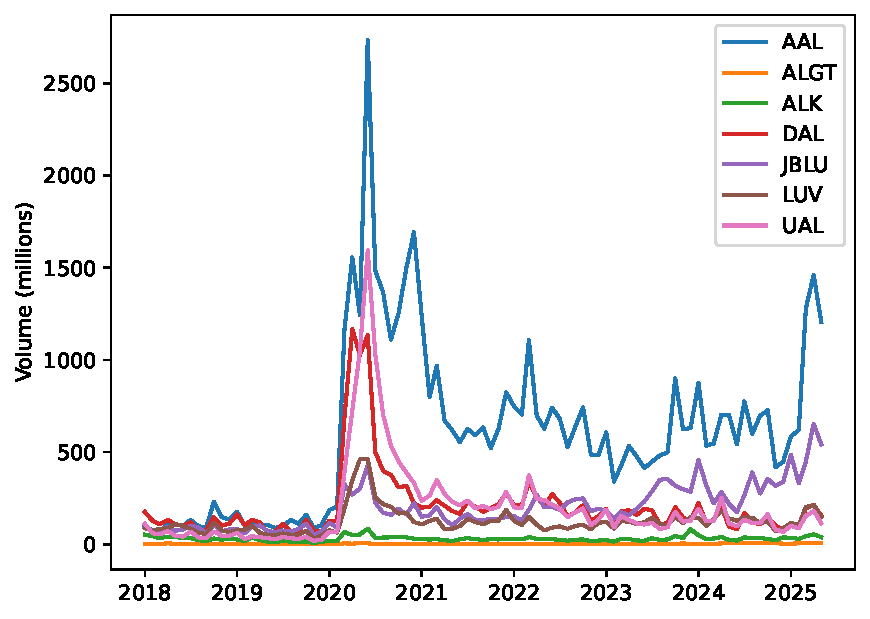
\includegraphics[width=0.7\linewidth]{../Output/monthly_volume_plot.pdf}
    \label{fig:monthly_volume}
\end{figure}

As an example of the potential usefulness of the GDELT data, we plot the trading volume and some sentiment measures for Alaskan Airlines on the two trading days before and after Jan. 5, 2024, when the window of a Boeing 737-9 plane blew open in flight.\footnote{\url{https://news.alaskaair.com/emergency-response/as-1282/}, \url{https://www.npr.org/2024/01/06/1223280562/alaska-airlines-flight-emergency-landing-oregon}.} The event happened on a Friday evening after regular trading hours, and so the stock volume does not react until Monday morning, Jan. 8. We can see in the figure below that trading volume on Monday morning sees a large spike compared to the prior two trading days, and this coincides with a clear shift in tone and article count for articles mentioning Alaska Airlines.
\begin{figure}[H]
    \centering
    \caption{Alaska Airlines Trading Volume and GDELT Sentiment Measures, Jan. 5, 2024}
    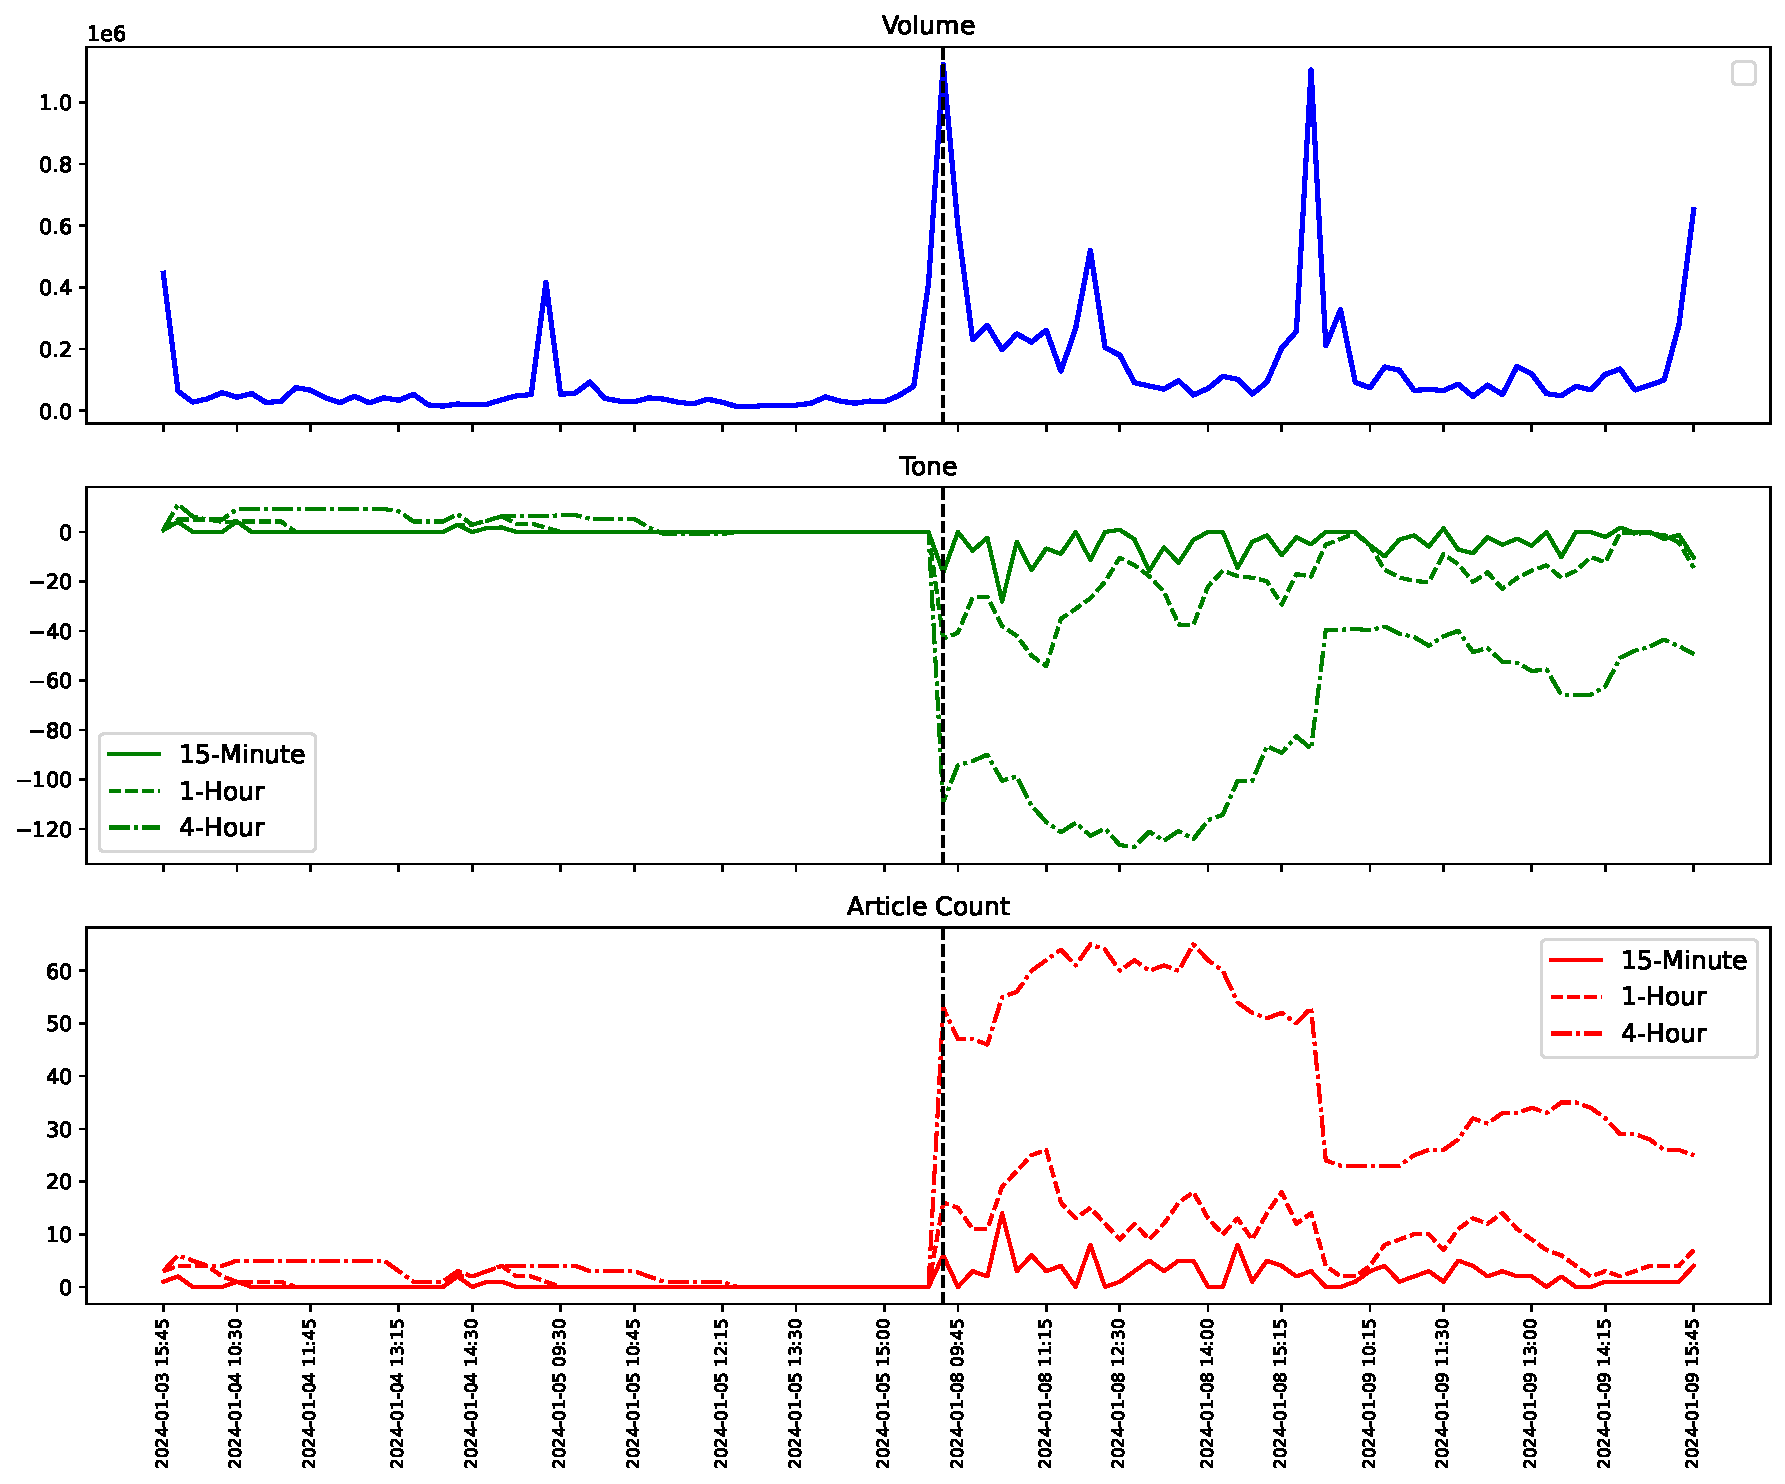
\includegraphics[width=0.9\linewidth]{../Output/alk_event_plot_52.pdf}
    \label{fig:alaska_volume_sentiment}
\end{figure}

\subsection{Correlation Analysis}
We can assess the usefulness of the GDELT sentiment measures on a broader scale by analyzing the correlation between stock volume and a 15-minute lag of some of the features. Figure \ref{fig:lagged_volume} reports a stock's current volume, price, and ``volume shock'' (change in volume compared to recent observations) in the columns, while each row is a selected sentiment measure from GDELT.\footnote{Specifically, volume shock is the difference between current volume and the 4-period moving average (lagged by 1 period) of volume.} Besides the typical sentiment measures, ``Oil Price'' and ``Earnings Report'' are word counts of articles mentioning the respective topic, and ``Sanctity (+) / Degradation (-)'' and ``Care (+) / Harm (-)'' are sentiment measures related to dimensions of morality.\footnote{According to \textcite{hopp2021extended}, the sanctity dimension measures moral disgust and spiritual concerns related to the body, while the care dimension involves intuitions of sympathy, compassion, and nurturance.} The results show that a higher article count, more polarity, and more positive \textit{or} negative words are all correlated with higher trading volume, but lower prices. The ``Oil Price'' and ``Earnings Report'' measures are also positively but weakly correlated with trading volume. The morality measures are negatively correlated with trading volume, i.e. when articles emphasize harm or moral disgust, trading volume tends to increase. The general reversal of correlations when looking at stock price is interesting. Finally, all correlations are much weaker when looking at  volume shock. This could suggest that prior trading volume absorbs much of the information reflected in the sentiment measures.

\begin{figure}[H]
    \centering
    \caption{Correlation of Trading Volume/Price and Lagged Sentiment Measures}
    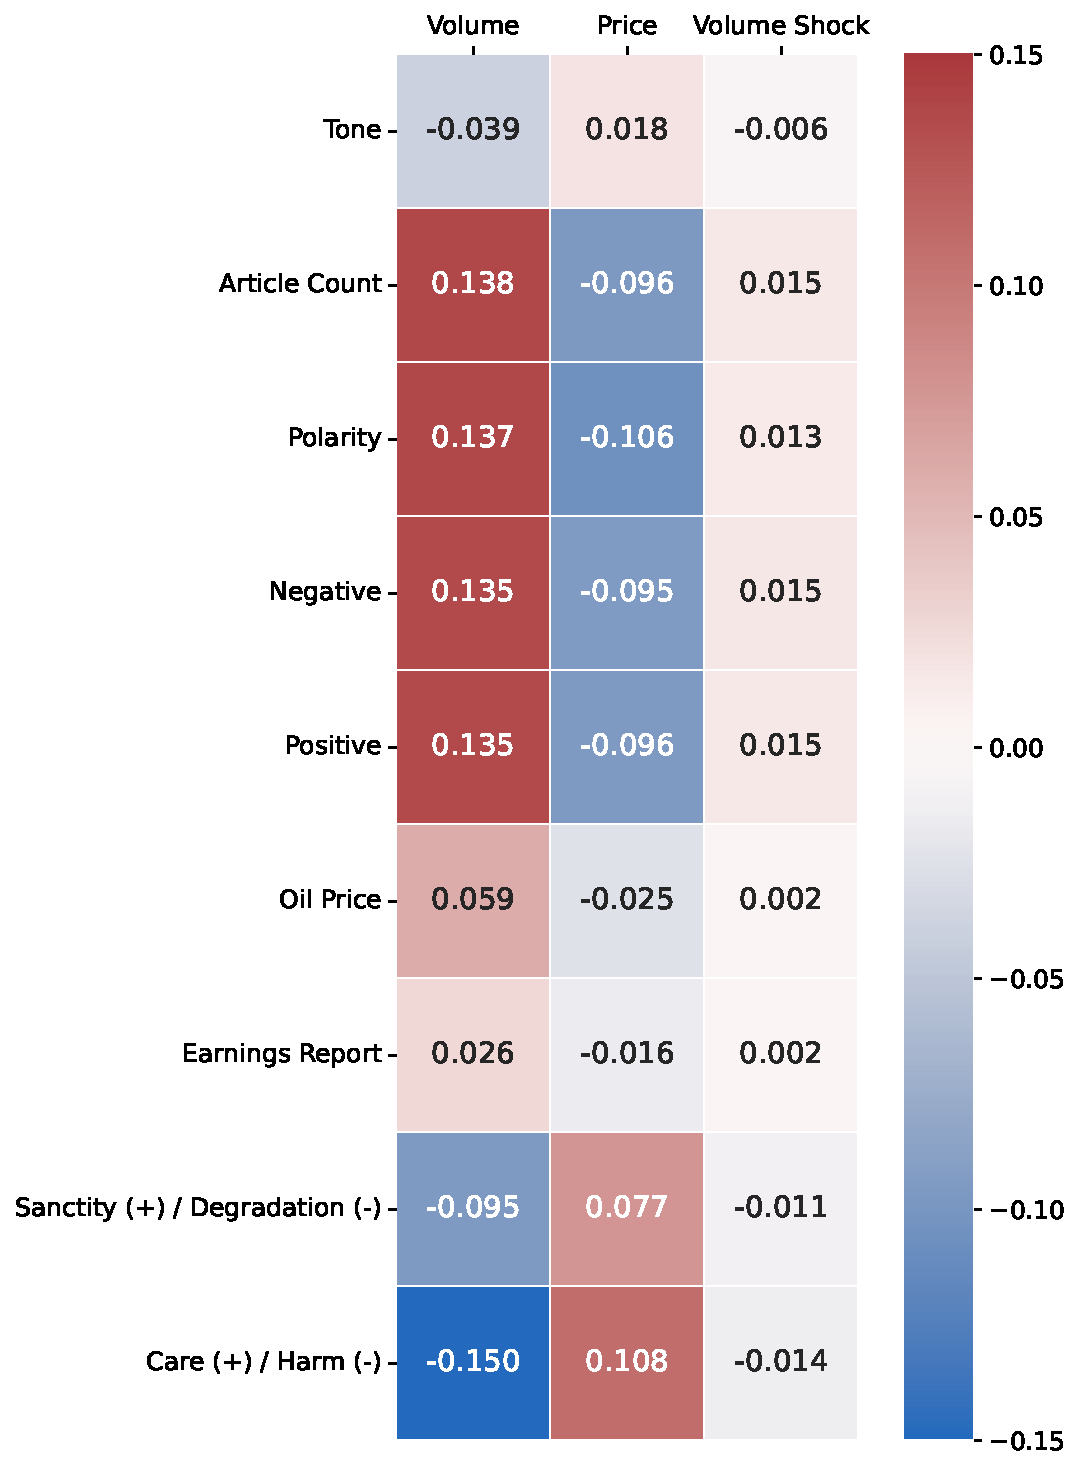
\includegraphics[width=0.6\linewidth]{../Output/correlations.pdf}
    \label{fig:lagged_volume}
\end{figure}

Trading volume is highly autocorrelated, periodic, and persistent, as discussed by \textcite{brownlees2011intra}. Figure \ref{fig:autocorrelations} reports the autocorrelations of the 15-minute trading volume as well as change in volume, where we have calculated the autocorrelation separately for each stock and then averaged the correlations. The gray area represents the minimum and maximum autocorrelation for any of the stocks at a given lag.

\begin{figure}[H]
    \centering
    \caption{Autocorrelations of Intraday Trading Volume}
    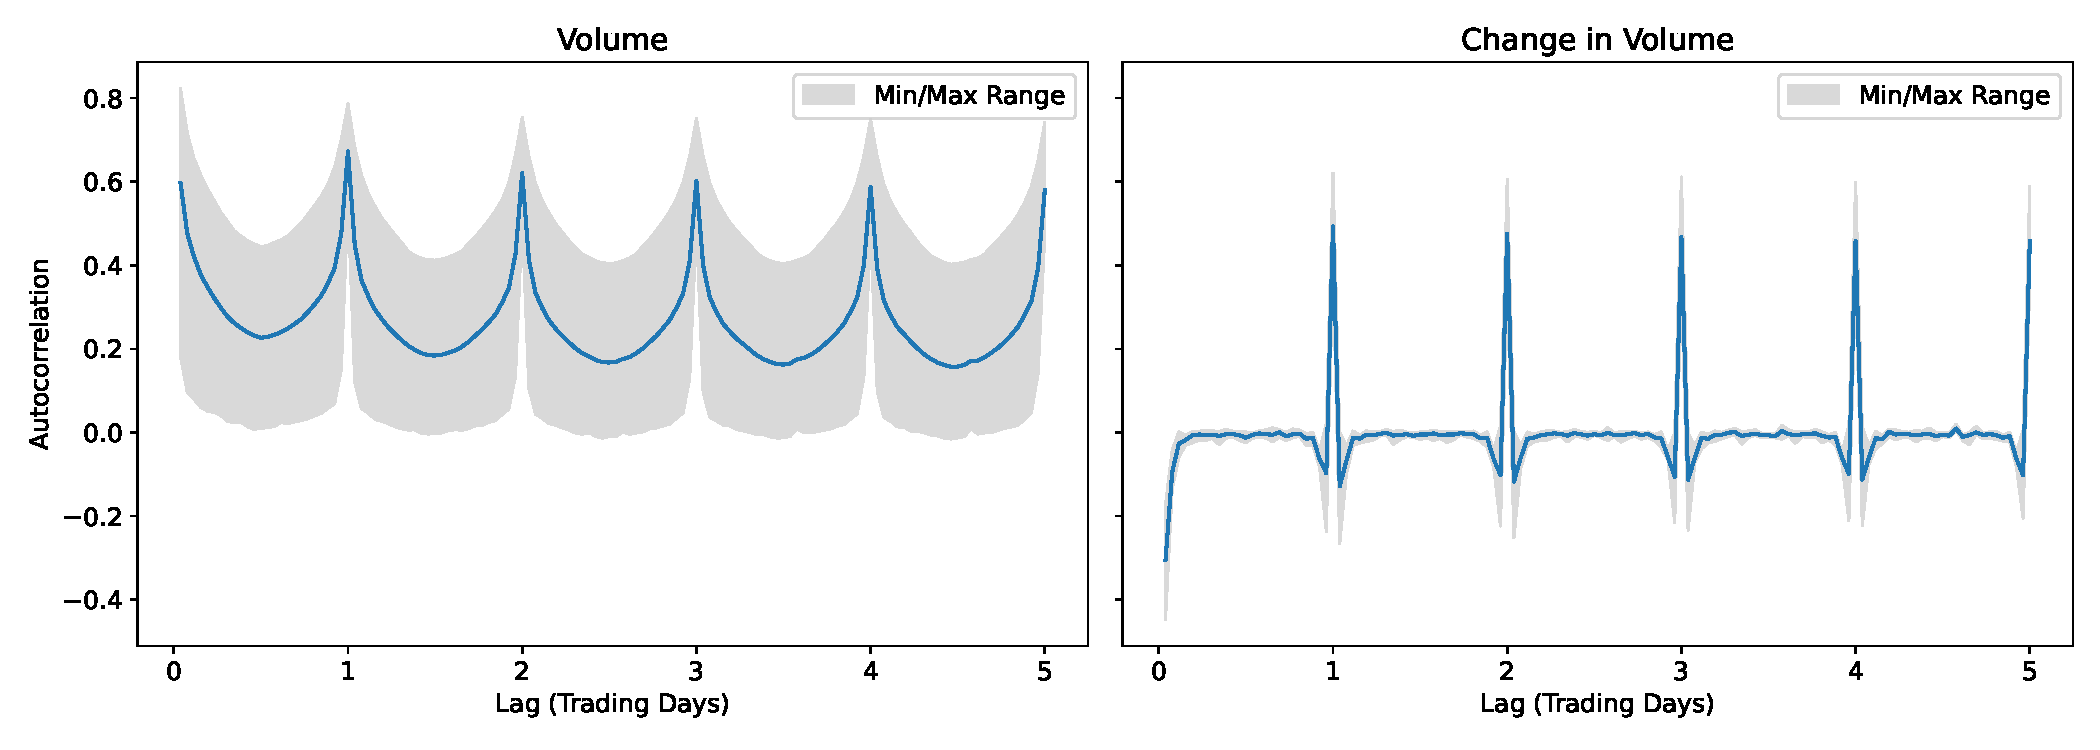
\includegraphics[width=\linewidth]{../Output/Volume Autocorrelations.pdf}
    \label{fig:autocorrelations}
\end{figure}

Stock volume autocorrelation has a consistent (and therefore predictable) pattern. Change in volume is negatively correlated with 15-minute lagged volume, has very little correlation to mid-day times, and is highly correlated with volume at the same time on previous days. We also see slight negative autocorrelation in the times just before and after a daily lag. The daily lagged correlation is highly persistent, with a 5-day lag having nearly as large of a correlation as the 1-day lag. 

\subsection{Models}
Before reporting the model results, we establish a baseline model. Similar to \textcite{goyenko2024trading}, we use a simple average of the trading volume for the past 5 days as a baseline predictor of volume.\footnote{Specifically, we use the 15-minute volume at the same time of the previous 5 trading days. Note that \textcite{goyenko2024trading} use the log-returns of dollar volume compared to a 5-day moving average, while we do not take logs.} This simple model performs quite well, with an out-of-sample $R^2$ of just under 0.55 over the entire testing period.

All models are evaluated using the out-of-sample $R^2$, described in the following formula:
\begin{equation}
    R^2 = 1 - \frac{\sum_{i\in O} (y_i - \hat{y}_i)^2}{\sum_{i\in O} (y_i - \bar{y}_i)^2}.
\end{equation}
In the formula, $O$ denotes the set of testing data, i.e. data that were not used in forming $\hat{y}$. One important aspect of the out-of-sample $R^2$ is that it is possible for models to have a negative $R^2$, if they perform worse than guessing the (out-of-sample) mean of the dependent variable.\footnote{While in-sample $R^2$ can also be negative in general, it is typically assumed to be non-negative. OLS models with a constant are guaranteed to have a non-negative in-sample $R^2$.}

\begin{table}[H]
\caption*{
{\large Out-of-Sample 15-Minute-Ahead Volume Prediction} \\
{\small $R^2$ Values, All Stocks, 2023-12-04 to 2025-05-30}
} 

\fontsize{12.0pt}{14.4pt}\selectfont

\begin{tabular*}{\linewidth}{@{\extracolsep{\fill}}lrrrr}
\toprule
Features & OLS & LASSO & Neural Network & LightGBM \\ 
\midrule\addlinespace[2.5pt]
Time Only & 0.0973 & 0.0973 & 0.0916 & 0.0978 \\
Sentiment Only & 0.0079 & 0.0314 & -0.0418 & 0.0762 \\
Self-Finance Only & 0.6330 & 0.6325 & 0.5912 & 0.6817 \\
Finance Only & 0.6361 & 0.6363 & 0.5702 & 0.6865 \\
Finance + Time & 0.6441 & 0.6444 & 0.6388 & 0.6893 \\
All & 0.6478 & 0.6492 & 0.6389 & 0.6952 \\
All (Tuned) &  &  &  & 0.7000 \\
All (Tuned, Retrained) &  &  &  & 0.7007 \\
\bottomrule
\end{tabular*}
\begin{minipage}{\linewidth}
Note: Models trained on data from 2018-01-02 to 2023-12-04.\\
\end{minipage}
\end{table}


Comparing the OLS and LASSO results shows that, besides the Sentiment Only feature set, the models provide similar performance. Surprisingly, however, the LASSO models consistently shrink a significant portion of coefficients: 392 of the 1576 features (nearly 25\%) are shrunk to zero in the model with all features.\footnote{Percentage of features shrunk to zero in the LASSO model by feature set: 0\% (Time Only), 9.9\% (Sentiment Only), 16.9\% (Own-Stock Only), 23.5\% (Market + Own-Stock), 24.3\% (Market + Own-Stock + Time), 24.9\% (All Features).} This suggests that the LASSO model identifies and removes a large number of features that do not contribute to the model's performance, although the features do not seem to hurt the OLS model's performance in general.

The Sentiment Only model results show that OLS and the Neural Network models are unable to effectively utilize sentiment information, with the Neural Network model having a negative $R^2$. The LASSO and LightGBM models have low but non-trivial out-of-sample performance, with the LightGBM model clearly performing best at over double the $R^2$ of the LASSO model. This suggests that the sentiment measures provide a small but non-trivial amount of information for predicting stock volume when harnessed correctly.

\subsection{Model Predictions}
All results in this section use the LightGBM model with the highest $R^2$ from the table above, unless otherwise specified.

First, we assess the model's out of sample performance on the validation and test sets (a combined 18 months of data) on a variety of subsets of the data. Figure \ref{fig:absolute_percent_error_distribution} reports the cumulative distribution of absolute percent error for the best model, as well as the baseline model. When plotted this way, a model is better at predicting volume if its cumulative distribution lies to the left of the other model's cumulative distribution. The figure shows that the LightGBM model is uniformly and significantly better than the baseline model on an absolute percent error basis.

\begin{figure}[H]
    \centering
    \caption{Absolute Percent Error Distribution}
    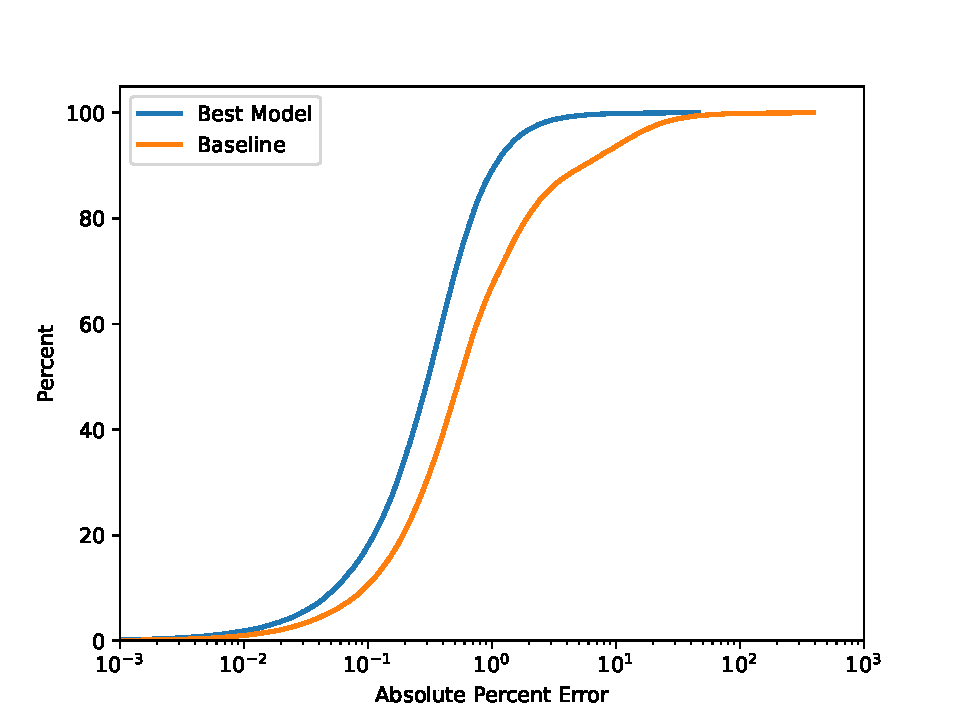
\includegraphics[width=0.75\linewidth]{../Output/absolute_percent_error_distribution.pdf}
    \label{fig:absolute_percent_error_distribution}
\end{figure}

Since stock volume can vary periodically, it is worth investigating the model's average performance at different times. Figure \ref{fig:mape_by_time} reports the mean absolute percent error (MAPE) by time of day.
\begin{figure}[H]
    \centering
    \caption{MAPE by Time of Day}
    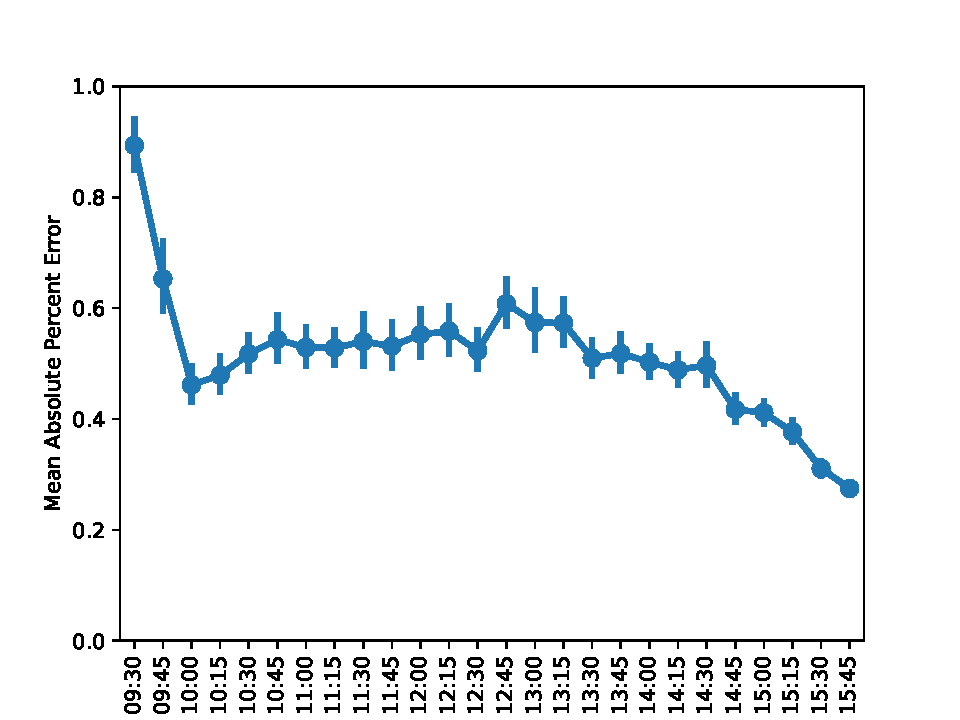
\includegraphics[width=0.75\linewidth]{../Output/mape_by_time.pdf}
    \label{fig:mape_by_time}
\end{figure}
The model is significantly worse at predicting volume in the first two periods of the trading day, which are highly volatile. The model is significantly better at predicting volume towards the end of the day; however, this is on a MAPE basis and so the results would differ on an absolute error basis (where end-of-day usually sees a spike in volume traded). Mid-day predictions are approximately of equal accuracy on average.

Figure \ref{fig:mape_by_time_by_ticker} breaks out the Figure above into individual tickers. This shows that the stocks generally share the same pattern described above, with some minor exceptions. ALGT is noticeably more variable than the other stocks, since its 95\% confidence intervals are wide and its MAPE is higher than the other stocks. This is likely due to ALGT's low trading volume, which makes it more difficult to predict. The other stocks generally have similar MAPE patterns, with the exception of JBLU, which has a much lower MAPE in the first two periods of the day. This suggests that JBLU's trading volume is more predictable in the early morning than the other stocks.
\begin{figure}[H]
    \centering
    \caption{MAPE by Time of Day and Ticker}
    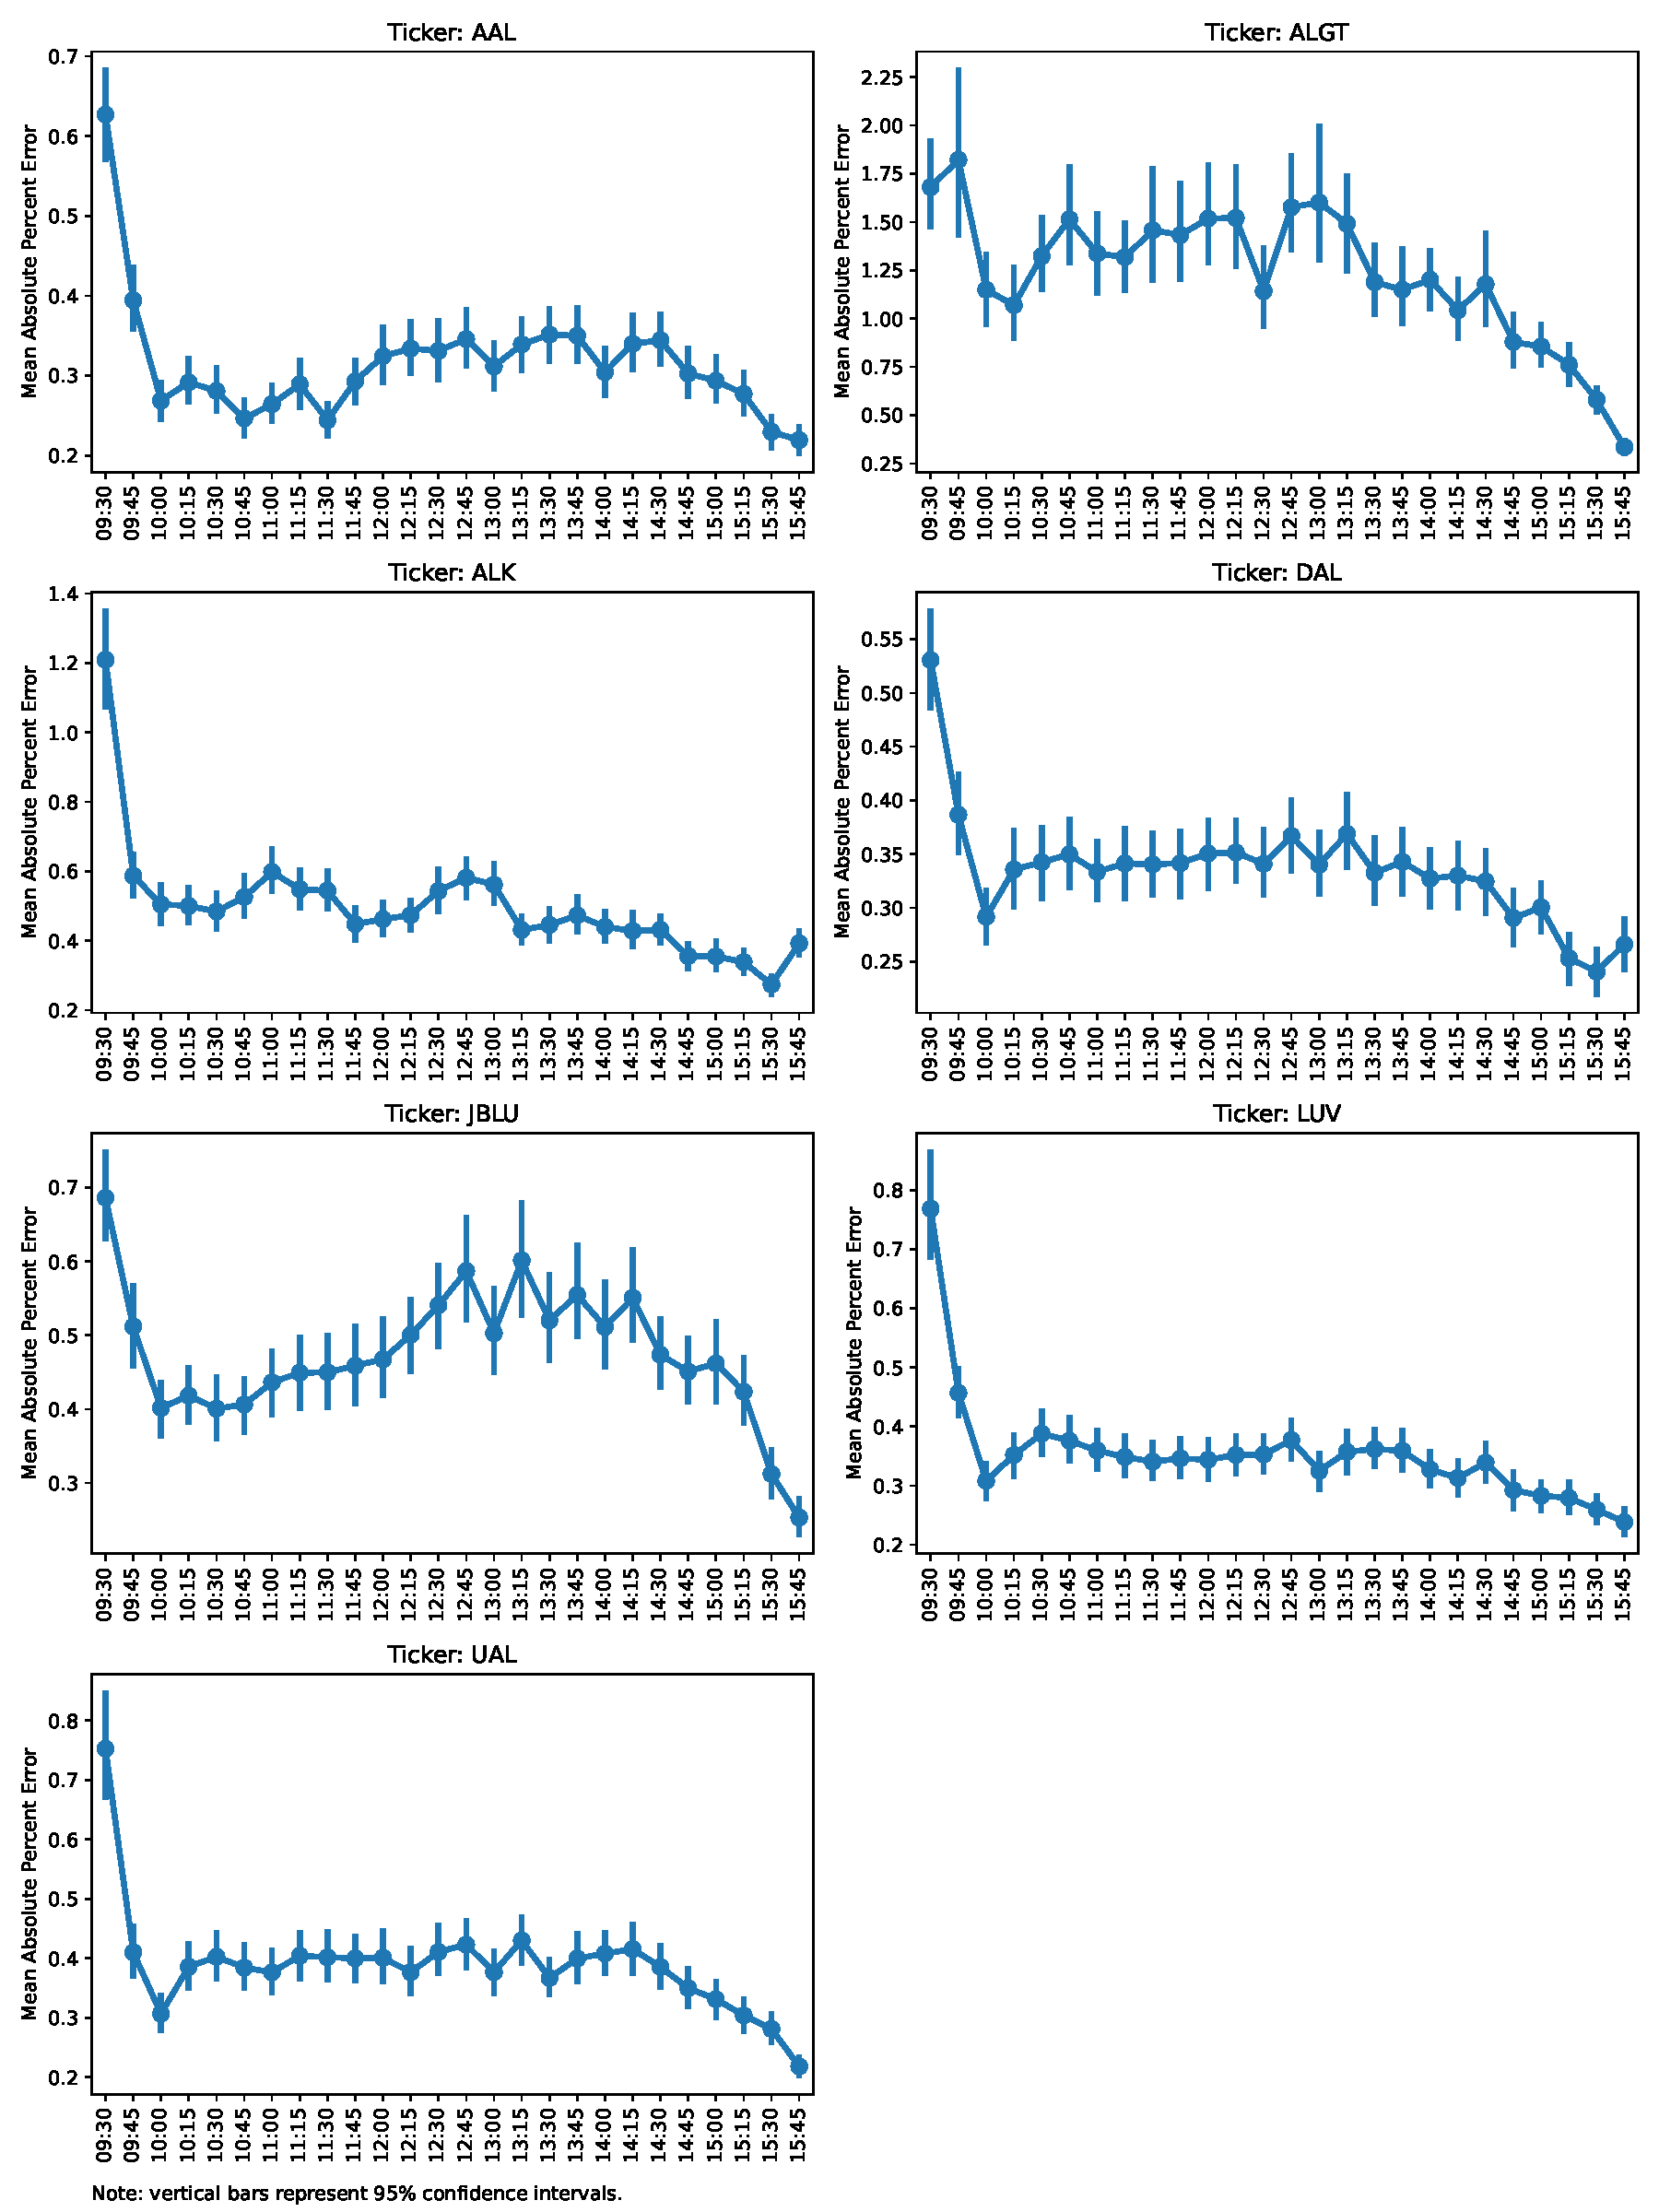
\includegraphics[width=0.75\linewidth]{../Output/mape_by_time_by_ticker.pdf}
    \label{fig:mape_by_time_by_ticker}
\end{figure}

Next, we assess the model's performance by day of week and day of month. Figure \ref{fig:mape_by_day_of_week} reports the MAPE by day of week, while Figure \ref{fig:mape_by_day_of_month} reports the MAPE by day of month. We see that the model is slightly less accurate on Mondays and Fridays, which is likely due to the fact that these days are more volatile than the other days of the week. The model also slightly decreases in performance as the month progresses, though there is much variance here.\footnote{Confidence intervals are not reported in this chart because they are very wide.}
\begin{figure}[H]
    \centering
    \caption{MAPE by Day of Week}
    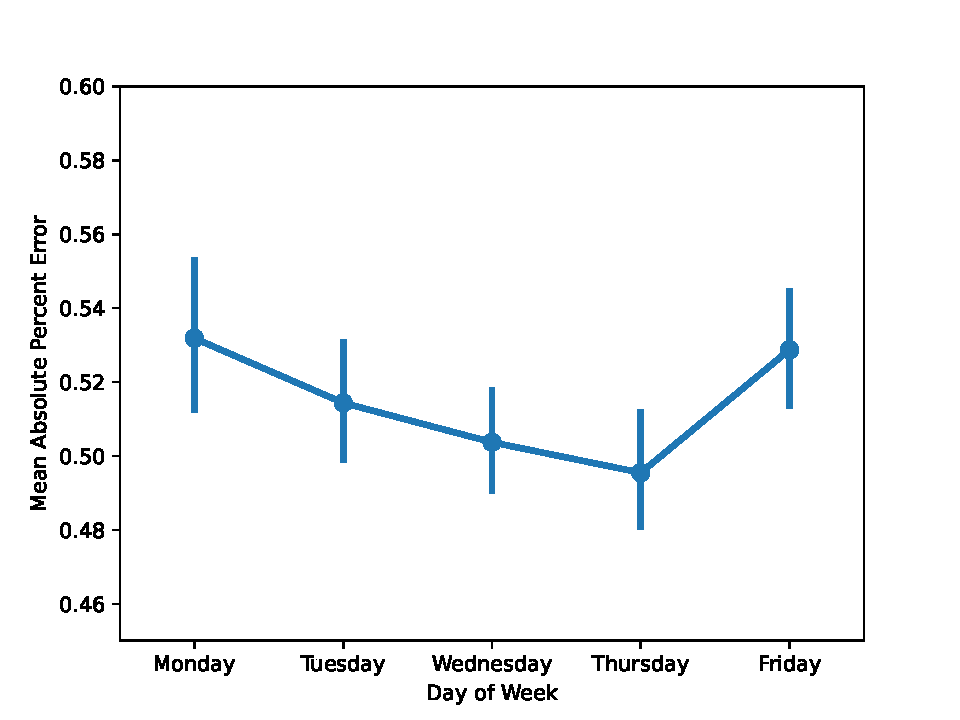
\includegraphics[width=0.75\linewidth]{../Output/mape_by_day_of_week.pdf}
    \label{fig:mape_by_day_of_week}
\end{figure}

\begin{figure}[H]
    \centering
    \caption{MAPE by Day of Month}
    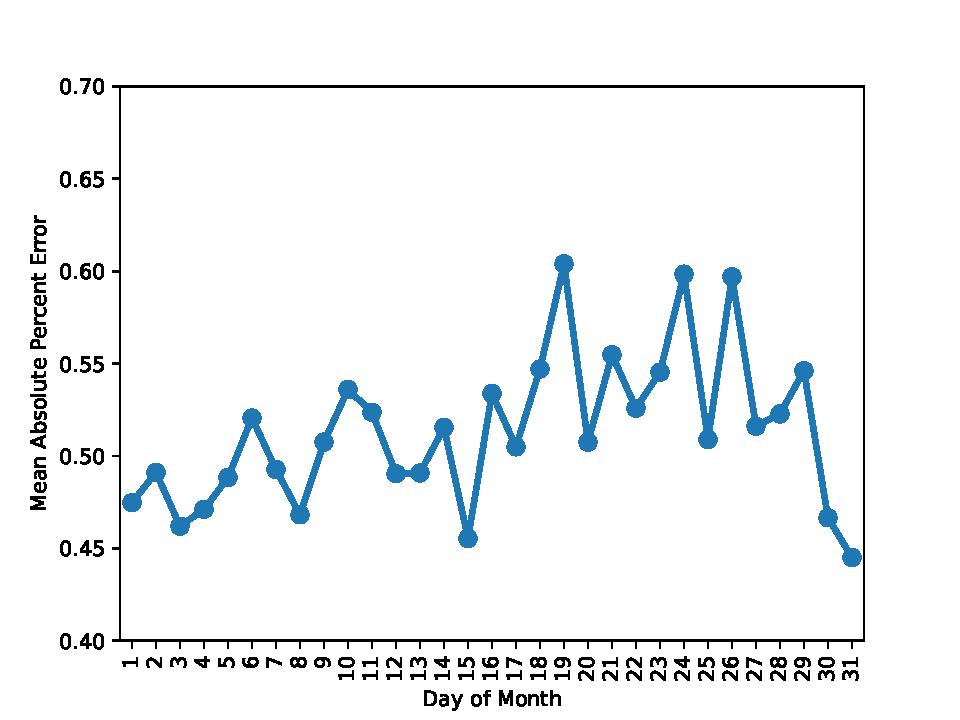
\includegraphics[width=0.75\linewidth]{../Output/mape_by_day_of_month.pdf}
    \label{fig:mape_by_day_of_month}
\end{figure}

\subsubsection{Sentiment Contribution}
We assess how important the sentiment measures are to the models' performance through the use of Shapley values.\footnote{We calculate Shapley values using a new, exact, tree-based method developed by \textcite{lundberg2020local2global}, as incorporated in the Python package \textsf{shap}.} Shapley values attribute the importance of each feature for a given model through the mechanics of cooperative game theory. Shapley values tell you by how much the given feature contributes the model's final prediction. For example, if a feature has a Shapley value of 100, then the model's prediction is 100 higher than it would be without that feature. A higher Shapley value (in absolute value) means that the feature contributes more to the model's predictions, meaning it is more important.

First, we report the mean absolute Shapley value for the top 20 most important features. These are the features that contribute most to the model's predicted volume, on average. Recall that because we scale all features to the interval $[0,1]$, Shapley values are comparable between features.
\begin{figure}[H]
    \centering
    \caption{Top 20 Features by Mean Absolute Shapley Value}
    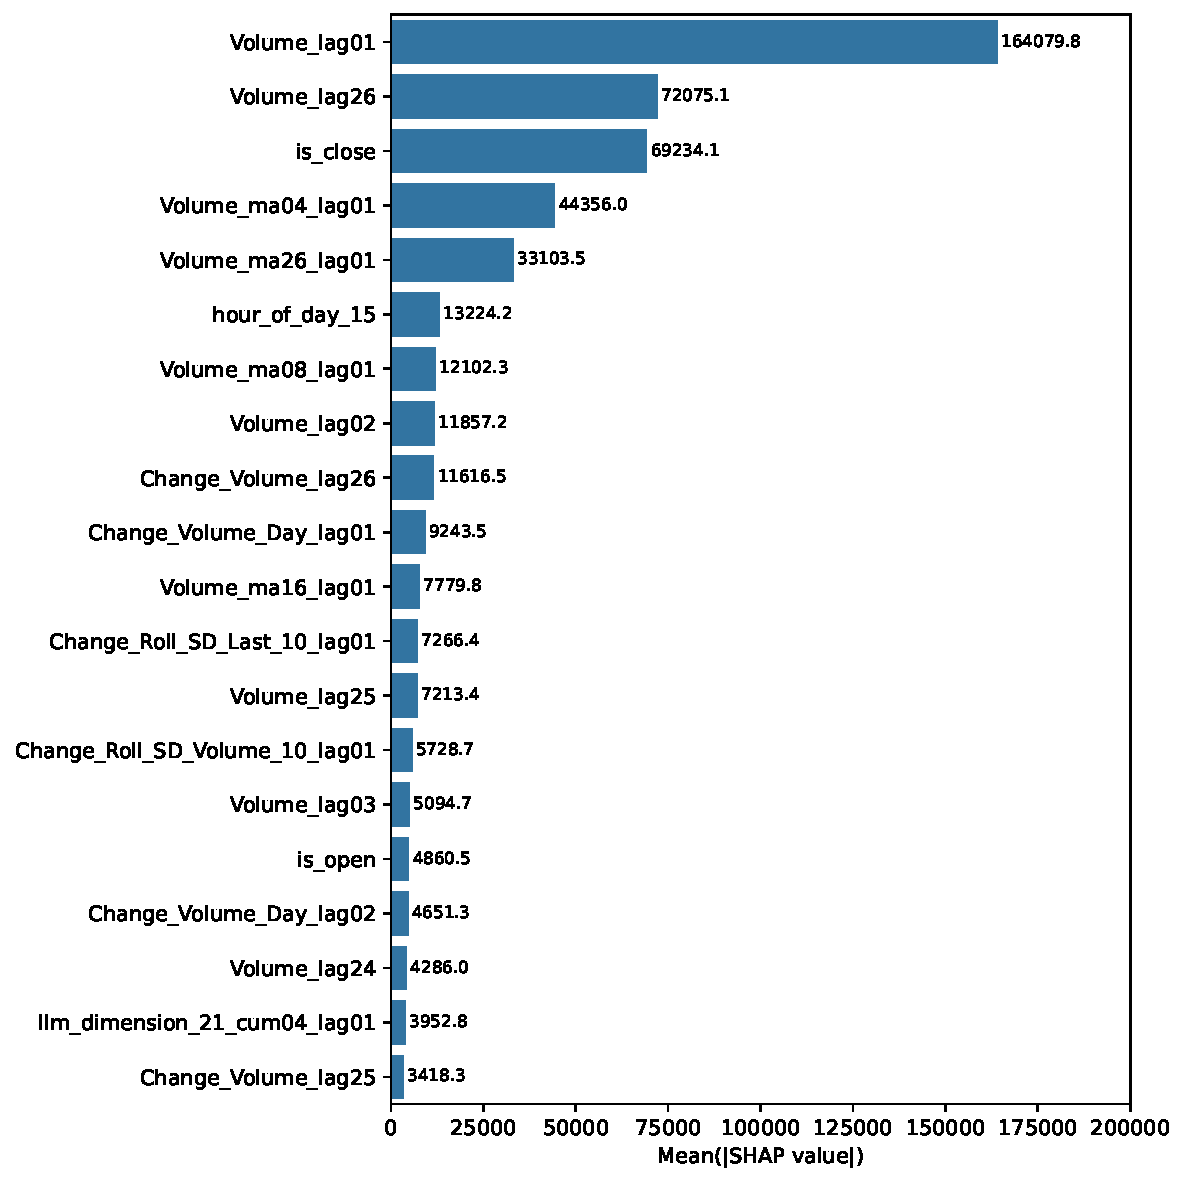
\includegraphics[width=0.75\linewidth]{../Output/shap_abs_all.pdf}
    \label{fig:shapley_overall}
\end{figure}

Unsurprisingly, the most important features are traditional financial and time indicators. The 15-minute lag of stock volume and 1 day (26-period) lag of volume are the most important features, followed by an indicator for whether the time is the last 15 minutes of the trading day. Moving average terms, differences in volume, and additional lags make up much of the top 20 most important features. However, one sentiment feature is included in the top 20: the 4-period cumulative sum of the 21st dimension of the headline LLM embedding.\footnote{LLM dimensions are 0-indexed, so feature name llm\_dimension\_21\_cum04\_lag01 actually refers to the 22nd dimension of the 32-dimensional LLM embedding vector.}

To further explore the sentiment features' contribution to the model, we report the mean absolute Shapley value for the sentiment features, sorted from highest to lowest.\footnote{Note that each sentiment variable has 5 features included: the original variable, and 4 cumulative sums of differing windows. We sum the Shapley values across these features to get its aggregate effect before taking the mean absolute value.} Figure \ref{fig:shapley_sentiment} reports the sentiment features that were shown above in the correlation analysis of Figure \ref{fig:lagged_volume}. As a reference point, the mean absolute Shapley value of the most important feature (the 15-minute lag of volume) is over 160,000.
\begin{figure}[H]
    \centering
    \caption{Selected GDELT Sentiment Variables, Mean Absolute Shapley Value}
    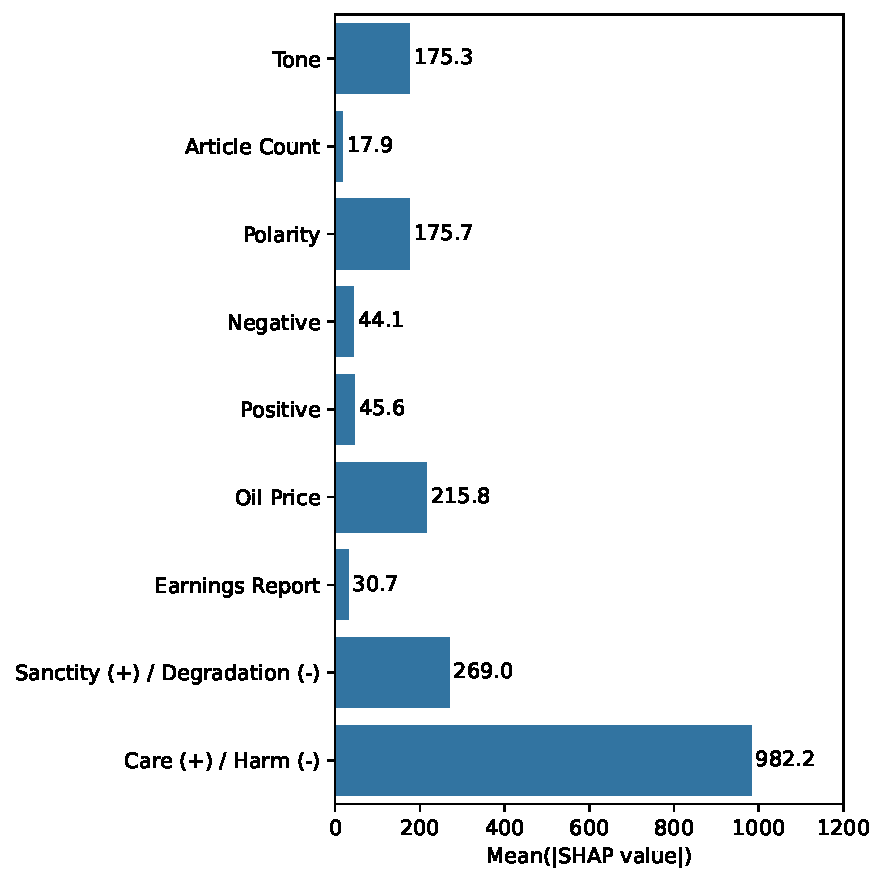
\includegraphics[width=0.75\linewidth]{../Output/shap_abs_sentiment.pdf}
    \label{fig:shapley_sentiment}
\end{figure}
Besides the Care/Harm moral sentiment feature, the remaining features contribute very little to the model's predictions on average. Figure \ref{fig:shapley_sentiment_top20} below shows the top 20 sentiment features, including the LLM dimensions, sorted by mean absolute Shapley value.

\begin{figure}[H]
    \centering
    \caption{Top 20 Sentiment Features by Mean Absolute Shapley Value}
    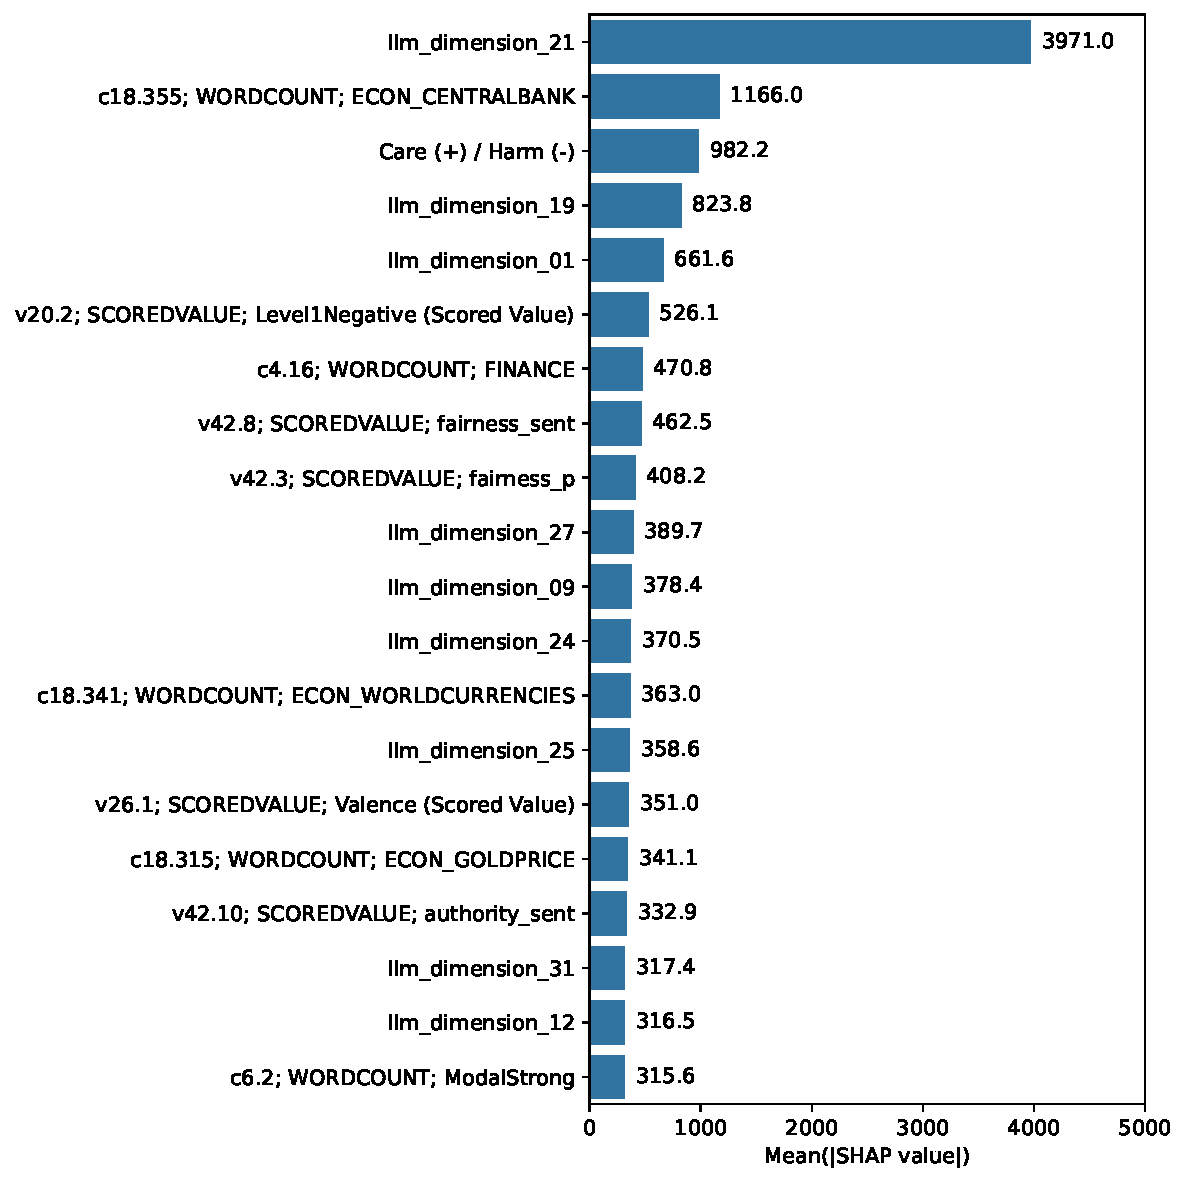
\includegraphics[width=0.75\linewidth]{../Output/shap_abs_sentiment_top20.pdf}
    \label{fig:shapley_sentiment_top20}
\end{figure}

There is a notable gap between the most important sentiment feature and the rest of the sentiment features. The most important sentiment feature is the 21st dimension of the headline LLM embedding as mentioned above, and the next most important feature (a word count for mentions of the Central Bank) has less than one third of its impact. It is also notable that the LLM dimensions often surpass the GDELT sentiment measures in importance.\footnote{We trained a LightGBM with all features except the LLM variables, and found an $R^2$ of 0.693, which is worse than simply not including the sentiment features.} 

As an additional study of the effects of sentiment on the model's predictions, we analyze how the model predicts volume for American Airlines surrounding the Jan. 2025 crash in Washington, D.C. that killed 67 people.\footnote{\url{https://apnews.com/article/ronald-reagan-national-airport-crash-325edc6c0c2439dd6c1e73a81e382c0e}.} Specifically, we look at the model's predictions of volume both with and without the effects of the sentiment features by removing their Shapley values.

\begin{figure}[H]
    \centering
    \caption{American Airlines Volume Predictions Surrounding Jan. 2025 Crash}
    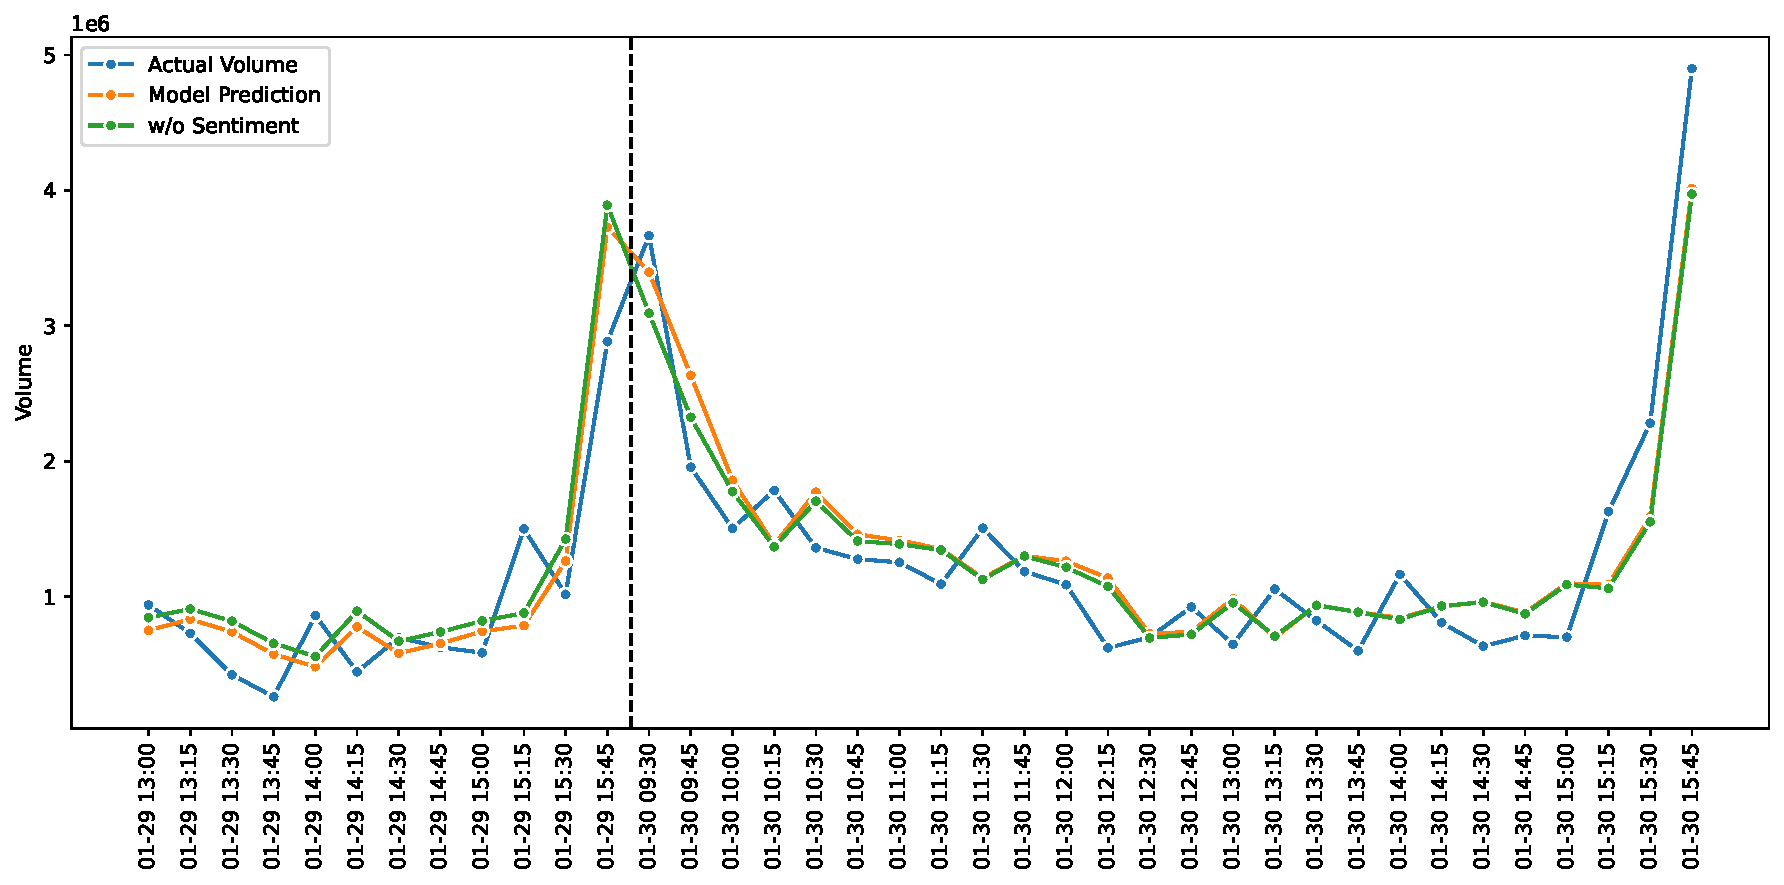
\includegraphics[width=\linewidth]{../Output/shap_aal_crash.pdf}
    \label{fig:shapley_aal_crash}
\end{figure}

The crash happened after the market had closed on Jan. 29, and so the news articles had been public for several hours before the market opened on Jan. 30.\footnote{There was significant after-hours trading of AAL on the morning of Jan. 30, which is not reflected in the figure. We chose not to include after-hours data in our analysis because most airlines hardly ever have any after-hours trading, but this is an example where it would have been helpful.} Even when analyzing what is likely the single most significant U.S. airline disaster during the entire data period, the model's predictions with and without sentiment features are nearly identical after the crash. The only differences are market open (9:30), where the model without sentiment features (green line) would have predicted slightly lower volume than when the features are included (orange line), and 9:45, where the sentiment features lead the model to overpredict volume. It is not at all obvious that the sentiment features provide meaningful value to the model's predictions, even in this extreme case.

Overall, it is clear that these sentiment measures add very little additional information to the model's predictions compared to the financial information.

\subsection{VWAP Tracking Error}
As discussed above, one of the primary uses of more accurate predictions of volume is to reduce the price impact of large trades: trades that comprise a significant proportion of total volume will have a higher price impact, which makes the trade more costly. Effectively forecasting volume would help the trader identify the right time to trade (i.e. when volume is high) to reduce those costs.

A full confirmation that the model reduces transaction costs would require us to actually make large trades in the market with and without the model, or to simulate such trades, as in \textcite{satish2014predicting}. We instead assess the LightGBM model's ability to reduce trading costs by comparing its VWAP tracking error to the baseline model's tracking error, following the approach described in \textcite{chen2016forecasting} and \textcite{cucuringu2025forecasting}. VWAP tracking error is defined as the absolute percent difference between the volume-weighted average price (VWAP) for stock $i$ at time $t$ and the stock's predicted VWAP at time $t$:
\begin{align}
    \text{VWAP}(i,t_0,t_1) &= \frac{\sum_{t=t_0}^{t_1} v_{it} \cdot p_{it}}{\sum_{t=t_0}^T v_{it}} \\
    \text{TE}_{it} &= \left| \frac{\text{VWAP}_{it} - \text{Predicted VWAP}_{it}}{\text{VWAP}_{it}} \right| \times 100\%
\end{align}

We use the last price in each 15-minute period for the VWAP formula. The lower the tracking error, the better the model is at predicting volume. Figure \ref{fig:vwap_tracking_error} shows the tracking error of the baseline model and the best model for each ticker. As can be seen, the LightGBM model provides a significant reduction in tracking error for each ticker, with the tracking error for DAL as low as 6.0 basis points (0.06\%). The largest proportional reduction in tracking error is for DAL as well with a 46.5\% reduction, while the smallest reduction is for ALGT at 11.1\%. A simple average across stocks yields an average improvement of \textbf{31.6\%} compared to the baseline model. In levels, the best model improves tracking error from 13.6 to 9.5 basis points, or \textbf{4.1} basis points on average. As stated by \textcite{chen2016forecasting}, for a broker with \$10 billion in turnover, saving just 1 basis point in trading costs would be worth \$1 million. 

\begin{figure}[H]
    \centering
    \caption{VWAP Tracking Error Comparison by Ticker}
    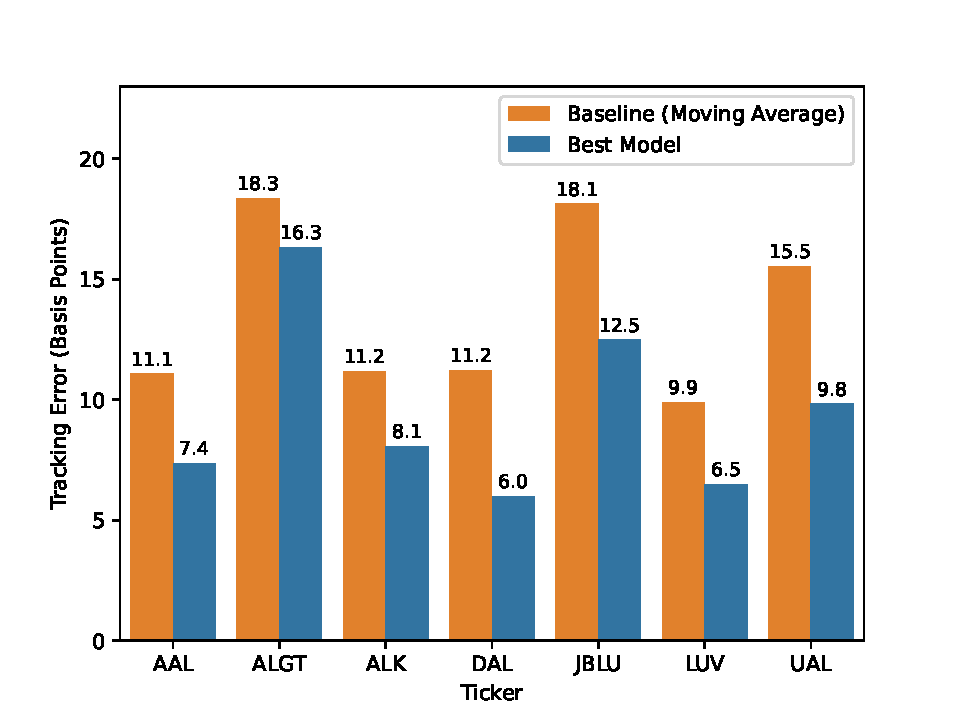
\includegraphics[width=0.85\linewidth]{../Output/vwap_compare.pdf}
    \label{fig:vwap_tracking_error}
\end{figure}

\newpage
\section{Discussion}
\label{section:discussion}
\subsection{Sentiment}
As shown in the table above, lagged sentiment features appear to provide some meaningful information in predicting stock volume, though it is a small contribution. First, a model run only with the sentiment features (Sentiment Only) has an out-of-sample $R^2$ of 0.0762 with the LightGBM model, which is roughly comparable to a model that only uses the time indicators (Time Only), with an $R^2$ of 0.0978.\footnote{We did not test the hypothesis that the Sentiment Only $R^2$ is greater than 0, but with the large size of the testing data, it is likely that the $R^2$ is statstically significant.}

As shown in the table above, adding the sentiment indicators improves each model's performance, but only marginally so. The best-performing model (LightGBM), improves its $R^2$ from 0.6893 to 0.6952 when incorporating the sentiment indicators into the model, not even a 1 percentage point increase. While it is an improvement, the lack of a large increase in performance suggests that historical financial data absorbs nearly all relevant sentiment information. While a financial institution seeking the most accurate forecasts may want to use GDELT's sentiment data as part of their volume forecasting, the data collection and curation costs are likely not worth the marginal increase in performance. On the contrary, the stock and other financial data are available at much lower cost and do not require the same level of curation.

\subsection{Model Performance Compared to the Literature}
In this section, we compare the various results reported above (and in our Appendix) to existing literature on stock volume prediction.

\textcite{cucuringu2025forecasting} model 15-minute intraday volume for a wide selection of stocks over a 6 month period. Their best model (a combination of convolutional and recurrent neural networks) achieves an out-of-sample $R^2$ of 0.624. Our best model instead yields an $R^2$ of 0.701 on a smalller set of stocks but over a much longer testing period. The authors were able to decrease VWAP tracking error by 28.7\% (2.1 basis points) on a sample of 5 stocks, while we decrease it by 31.6\% (4.1 basis points) on our stocks.\footnote{We use a different baseline model than \textcite{cucuringu2025forecasting}, and our errors are larger in levels compared to them. However, the authors did not analyze our stocks specifically, so these results are not fully comparable.}

\textcite{chen2016forecasting} predict 15-minute trading volume for 30 international securities over a 1-year testing period. Their best model achieves an out-of-sample mean absolute percent error (MAPE) of 0.46, a 29\% improvement over their baseline model. Our best model has a MAPE of 0.515 over a 1.5-year testing period, an improvement of 24\% over our baseline.\footnote{See Appendix, Section \ref{section:appendix_model_performance}.} The authors' best model has an average VWAP tracking error of 6.38 basis points, a 9\% improvement over the baseline. Our best model has a tracking error of 9.5 basis points, a 31.6\% improvement over our baseline.\footnote{Again, we use a different baseline model and different stocks, so these results are not fully comparable.}

\textcite{satish2014predicting} use a combination of ARMA models to predict 15-minute trading volume for 500 stocks over 250 trading days, finding that their best model improves the median absolute percentage error of volume by 24\% over a baseline model. Our best model reduces median error by 26\%. The authors were able to reduce VWAP tracking error in a large-scale trading simulation study by 9.1\%, to 8.74 basis points, while our best model reduces tracking error by 31.6\% (9.5 basis points).

\subsection{Limitations and Suggestions for Future Work}
The main limitation of this work is that we only analyze 7 stocks. This is due to the computational expense of gathering and processing the GDELT data, which is required to use the sentiment features. It is quite possible that certain companies, industries, or currencies would benefit more from sentiment features than the airline industry, which is why we recommend future work to analyze a wider variety of stocks and industries. Researchers could substantially reduce the time to gather GDELT data by using Google BigQuery to extract the data, but this comes with computing costs on the order of thousands to tens of thousands of dollars.

We identified relevant sentiment features using judgement and experimentation, and so it is possible that additional features could have improved the models' performance. In particular, we only include the sentiment of articles that specifically mention the airlines of interest. Other news topics (such as weather, politics, or the economy) may also be informative for predicting stock volume, and so future work could include these features as well. Additionally, GDELT does not include certain news sources that would be helpful, such as SEC filings or earnings call transcripts. Incorporating sentiment from earnings calls would very likely improve the model's performance.

Since influential news events are typically rare for a specific company, including the sentiment features along with the finance features in a single model may not have been optimal. A better approach might have been to train a baseline model on financial features, and then train a separate model to identify the impact of sentiment on volume, i.e. as a modifier.

\section{Conclusion}
\label{section:conclusion}
The model results confirm that stock volume can be accurately forecasted better than a baseline model using historical averages. However, the results also show that sentiment measures add little additional content beyond historical financial information. This suggests that costly sentiment data curation may not be necessary for better-than-baseline stock volume prediction. However, financial institutions seeking the absolute best performance may want to include sentiment measures to get a small boost in forecasting accuracy.

\newpage
\printbibliography
\newpage

\section{Appendix}
\subsection{Model Performance}
\label{section:appendix_model_performance}
A table showing the MAPE for each model tested is shown below. The baseline model has a MAPE of 0.678.
\begin{table}[H]
\caption{
{ Out-of-Sample MAPE, 15-Minute-Ahead Volume Prediction} \\
{\small All Stocks, 2023-12-04 to 2025-05-30}
} 

\fontsize{12.0pt}{14.4pt}\selectfont

\begin{tabular*}{\linewidth}{@{\extracolsep{\fill}}lrrrr}
\toprule
Features & OLS & LASSO & Neural Network & LightGBM \\ 
\midrule\addlinespace[2.5pt]
Time Only & 18.048 & 18.049 & 18.407 & 18.015 \\
Sentiment Only & 5.198 & 5.040 & 6.407 & 9.286 \\
Self-Finance Only & 1.066 & 1.038 & 1.479 & 0.504 \\
Finance Only & 2.173 & 1.870 & 1.262 & 0.534 \\
Finance + Time & 2.123 & 1.878 & 1.011 & 0.527 \\
All & 2.113 & 1.783 & 1.641 & 0.516 \\
All (Tuned) &  &  &  & 0.566 \\
All (Tuned, Retrained) &  &  &  & 0.515 \\
\bottomrule
\end{tabular*}
\begin{minipage}{\linewidth}
Note: Models trained on data from 2018-01-02 to 2023-12-04.\\
\end{minipage}
\end{table}


\subsubsection{Alternative Model Specification}
It is worth questioning whether, instead of predicting volume, the model would do better by predicting a normalized change in volume and then rescaling the predictions. We tried a similar method to \textcite{goyenko2024trading}, where we predict the change in volume compared to the baseline model's prediction. In testing the LightGBM model on the different feature sets, we found that these models do not improve the prediction of volume: using all features yields an $R^2$ of 0.6450, which is worse than our original model. Attempts to use the sentiment features alone or time features alone yielded models that predict volume worse than the baseline model.

\subsubsection{Current Sentiment Model}
One way to test assess the upper limit of the sentiment features' ability to explain stock volume is to model volume as a function of \textit{current} sentiment, rather than lagged sentiment. This is an ``oracle''-style model, in that the model is infeasible for predictive purposes but informative for understanding the maximum usefulness of the features. We trained a LightGBM model predicting current volume with all sentiment features, with the following parameters: learning rate 0.01, min. samples per leaf 200, L2 regularization 0, max. features 1. The model has an out-of-sample $R^2$ of 0.0883, which is around 15\% better than the lagged model reported in our main results above. This suggests both that the sentiment features provide only a limited amount of useful information about volume, and that the 15-minute lagged features provide nearly as much information as they possibly could.

\subsection{GDELT Data Processing}
\label{section:gdelt_details}
Additional detail on GDELT data processing is provided below. For even further detail, we recommend viewing our source code in the GitHub repository linked in the introduction.

GDELT offers a variety of databases to the public. For this analysis, we use the Global Knowledge Graph (GKG), version 2.\footnote{\url{https://blog.gdeltproject.org/gdelt-2-0-our-global-world-in-realtime/}.} For each article identified by GDELT, the GKG data includes:
\begin{itemize}
\singlespacing
    \item the date scraped by GDELT (at the 15-minute level)
    \item the article URL (or other unique identifier)
    \item every location, business, and important person named in the article text
    \item A wide variety of sentiment measures based on the article text
    \item the article headline text (if available).\footnote{GDELT only started scraping the article headline in Sep. 2019. Prior to this time, we recover part of the article headline using the URL, which often contains a relevant description of the story.}
\end{itemize}
GDELT uploads GKG data in separate files every 15 minutes. These files are available to download for free, but the full combined data is available to query in Google BigQuery for a fee. The files are saved at the article level, i.e. the articles that GDELT scraped in a given 15-minute period.

Because the combined data is several tens of terabytes (TBs), we did not have the storage capacity to save all the raw data. Instead, we filtered the raw files to articles matching the airline industry before saving the data. The general outline of our data processing is:
\begin{itemize}
\singlespacing
    \item access and unzip the raw file for a given 15-minute period
    \item keep a limited subset of columns from the raw file
    \item limit to articles mentioning a location of ``United States"
    \item limit to articles that mention at least one of the following organizations: Alaska Airlines, American Airlines, Delta Air Lines, Frontier Airlines, Hawaiian Airlines, JetBlue, Southwest Airlines, Spirit Airlines, Sun Country Airlines, United Airlines, Allegiant Air
    \item drop articles that are missing any key fields
\end{itemize}
We repeated this process for the approximately 260,000 15-minute periods covering the timeline of 1/1/2018 00:00:00 to 5/30/2025 23:45:00. Data downloading was performed over multiple several-hour periods, and was parallelized to increase download speeds. After filtering, 218,574 raw GDELT files were combined for a total of 1,261,785 articles identified.\footnote{The total raw GDELT files kept is less than the theoretical 260,000 files for multiple reasons, including: no airlines mentioned in the past 15 minutes, and sporadic GDELT outages.}

Next, we performed extensive data cleaning to filter the articles to those that would likely affect the stock market:
\begin{itemize}
\singlespacing
    \item restricting the sentiment indicators to finance- and economics-specific measures
    \item removing frequent article titles that relate to the front page of a news site (rather than a specific article) or an unrelated article
    \item restricting to top news websites (e.g. MSN, Reuters) and finance-related websites (e.g. Investors.com)
    \item removing discussions of historical airline events (such as the September 11 attacks)
    \item removing articles that did not have a valid article title after data processing
    \item removing a small set of duplicate articles\footnote{Duplicate articles are likely due to the data downloading process, which was stopped and restarted multiple times.}
\end{itemize}
After cleaning and filtering, we have 121,655 relevant articles and 118 sentiment measures.

To extract additional sentiment from the GDELT data, we use a \textbf{Large Language Model} (LLM) to embed the article titles in a high-dimensional vector space. We apply a 596-million parameter embedding model to each article title.\footnote{\url{https://huggingface.co/Qwen/Qwen3-Embedding-0.6B}. This embedding model optionally takes an instruction prompt as an input. We use the following prompt for our embeddings: \textsf{Instruct: Extract the sentiment from this news headline that is most likely to affect the airline stock market. Query:}.} The model is trained to output 1024-dimensional vectors, however we use the Matryoshka Transformer (MatFormer) method to truncate the vectors to 32 dimensions, acting as a dimensionality reduction technique. These 32 dimensions are then used as additional sentiment measures in the model.

After constructing the sentiment measures, we aggregate the data to align with stock market data and to identify sentiment scores separately by airline. Each metric is interacted with a set of indicator variables identifying the airline companies.\footnote{Multiple airlines can be mentioned in the same article, in which case the article is included each of the airlines' interacted sentiment values.} We then sum the metrics by 15-minute interval and fill in missing time periods with zeroes.\footnote{GDELT data is recorded in the UTC timezone, while my stock data is in EST. I converted the timezone before merging these datasets.} At this point, the GDELT data is in 15-minute intervals, but it includes times outside of market open. We further aggregate the data to align with market open. The choice of aggregation strategy is not obvious here. The number of observations to aggregate influences the scale of the resulting sentiment scores. Summing a particular window of observations (e.g. 2 hours) assumes that sufficient information is captured in that time period for predicting stock behavior.\footnote{Note that simply collapsing all of the market close data into one observation would result in large sentiment values at market open, and small values for the rest of the trading day. This would essentially vanish any effects of events that occur during the trading day.} We address this issue by calculating rolling sums over varying time windows: 1 hour, 4 hours, 12 hours, and 24 hours. These sums influence the non-after-hours observations as well, making them essentially moving averages. Each of these rolling sums is included in the feature set to allow the model to identify combinations of windows that best fit the data.

After calculating the rolling sums for each airline, metric, and window, we calculate the first lag of each variable to ensure that they can be used for out-of-sample predictions. Finally, the data is reshaped so that each observation is a 15-minute-bin and stock ticker. The final data has 338,324 rows and 750 sentiment features.

\subsection{Sentiment Measures}
A complete list of the sentiment measures selected from GDELT's GKG is given below, along with their sources as reported by GDELT.\footnote{\url{http://data.gdeltproject.org/documentation/GCAM-MASTER-CODEBOOK.TXT}.}

\footnotesize
\begin{verbatim}
c16.60, WORDCOUNT, WordNet Domains 3.2, finance
c18.1, WORDCOUNT, GDELT GKG Themes, KILL
c18.121, WORDCOUNT, GDELT GKG Themes, UNSAFE_WORK_ENVIRONMENT
c18.137, WORDCOUNT, GDELT GKG Themes, TRIAL
c18.154, WORDCOUNT, GDELT GKG Themes, ECON_MONOPOLY
c18.157, WORDCOUNT, GDELT GKG Themes, AVIATION_INCIDENT
c18.164, WORDCOUNT, GDELT GKG Themes, CORRUPTION
c18.178, WORDCOUNT, GDELT GKG Themes, ECON_ENTREPRENEURSHIP
c18.187, WORDCOUNT, GDELT GKG Themes, ECON_SUBSIDIES
c18.188, WORDCOUNT, GDELT GKG Themes, ECON_DEREGULATION
c18.189, WORDCOUNT, GDELT GKG Themes, ECON_NATIONALIZE
c18.2, WORDCOUNT, GDELT GKG Themes, WOUND
c18.21, WORDCOUNT, GDELT GKG Themes, LEGISLATION
c18.213, WORDCOUNT, GDELT GKG Themes, ECON_TAXATION
c18.214, WORDCOUNT, GDELT GKG Themes, ECON_REMITTANCE
c18.215, WORDCOUNT, GDELT GKG Themes, ECON_INFORMAL_ECONOMY
c18.223, WORDCOUNT, GDELT GKG Themes, ECON_DEBT
c18.246, WORDCOUNT, GDELT GKG Themes, ECON_FREETRADE
c18.247, WORDCOUNT, GDELT GKG Themes, ECON_FOREIGNINVEST
c18.248, WORDCOUNT, GDELT GKG Themes, ECON_PRICECONTROL
c18.254, WORDCOUNT, GDELT GKG Themes, ACT_MAKESTATEMENT
c18.258, WORDCOUNT, GDELT GKG Themes, ECON_BOYCOTT
c18.279, WORDCOUNT, GDELT GKG Themes, ECON_MOU
c18.280, WORDCOUNT, GDELT GKG Themes, ECON_CUTOUTLOOK
c18.286, WORDCOUNT, GDELT GKG Themes, ECON_BUBBLE
c18.287, WORDCOUNT, GDELT GKG Themes, ECON_INFLATION
c18.288, WORDCOUNT, GDELT GKG Themes, ECON_DEFLATION
c18.289, WORDCOUNT, GDELT GKG Themes, ECON_UNDEREMPLOYMENT
c18.290, WORDCOUNT, GDELT GKG Themes, ECON_IDENTITYTHEFT
c18.292, WORDCOUNT, GDELT GKG Themes, ECON_MIDDLECLASS
c18.293, WORDCOUNT, GDELT GKG Themes, ECON_WORKINGCLASS
c18.294, WORDCOUNT, GDELT GKG Themes, ECON_EMERGINGECON
c18.30, WORDCOUNT, GDELT GKG Themes, WHISTLEBLOWER
c18.307, WORDCOUNT, GDELT GKG Themes, ECON_COUNTERFEITMONEY
c18.314, WORDCOUNT, GDELT GKG Themes, ECON_OILPRICE
c18.315, WORDCOUNT, GDELT GKG Themes, ECON_GOLDPRICE
c18.316, WORDCOUNT, GDELT GKG Themes, ECON_GASOLINEPRICE
c18.317, WORDCOUNT, GDELT GKG Themes, ECON_HEATINGOIL
c18.318, WORDCOUNT, GDELT GKG Themes, ECON_HEATINGOILPRICE
c18.319, WORDCOUNT, GDELT GKG Themes, ECON_DIESELPRICE
c18.320, WORDCOUNT, GDELT GKG Themes, ECON_HEATINGOIL
c18.321, WORDCOUNT, GDELT GKG Themes, ECON_PROPANE
c18.323, WORDCOUNT, GDELT GKG Themes, ECON_ELECTRICALGENERATION
c18.324, WORDCOUNT, GDELT GKG Themes, ECON_ELECTRICALGRID
c18.325, WORDCOUNT, GDELT GKG Themes, ECON_ELECTRICALDEMAND
c18.326, WORDCOUNT, GDELT GKG Themes, ECON_ELECTRICALLOADSHEDDING
c18.327, WORDCOUNT, GDELT GKG Themes, ECON_ELECTRICALPRICE
c18.328, WORDCOUNT, GDELT GKG Themes, ECON_NEWPOWERPLANT
c18.329, WORDCOUNT, GDELT GKG Themes, ECON_NATGASPRICE
c18.33, WORDCOUNT, GDELT GKG Themes, DELAY
c18.332, WORDCOUNT, GDELT GKG Themes, ECON_PRICEGOUGE
c18.336, WORDCOUNT, GDELT GKG Themes, ECON_MONEYLAUNDERING
c18.337, WORDCOUNT, GDELT GKG Themes, ECON_BITCOIN
c18.340, WORDCOUNT, GDELT GKG Themes, ECON_FOREIGNBANKS
c18.341, WORDCOUNT, GDELT GKG Themes, ECON_WORLDCURRENCIES
c18.355, WORDCOUNT, GDELT GKG Themes, ECON_CENTRALBANK
c18.36, WORDCOUNT, GDELT GKG Themes, ECON_DEVELOPMENTORGS
c18.42, WORDCOUNT, GDELT GKG Themes, ECON_COST_OF_LIVING
c18.47, WORDCOUNT, GDELT GKG Themes, ECON_TRADE_DISPUTE
c18.50, WORDCOUNT, GDELT GKG Themes, SHORTAGE
c18.53, WORDCOUNT, GDELT GKG Themes, ECON_UNIONS
c18.54, WORDCOUNT, GDELT GKG Themes, ECON_BANKRUPTCY
c18.57, WORDCOUNT, GDELT GKG Themes, ECON_CURRENCY_RESERVES
c18.58, WORDCOUNT, GDELT GKG Themes, ECON_CURRENCY_EXCHANGE_RATE
c18.59, WORDCOUNT, GDELT GKG Themes, ECON_STOCKMARKET
c18.60, WORDCOUNT, GDELT GKG Themes, ECON_EARNINGSREPORT
c18.61, WORDCOUNT, GDELT GKG Themes, ECON_IPO
c18.62, WORDCOUNT, GDELT GKG Themes, ECON_HOUSING_PRICES
c18.63, WORDCOUNT, GDELT GKG Themes, ECON_INTEREST_RATES
c18.66, WORDCOUNT, GDELT GKG Themes, STRIKE
c18.68, WORDCOUNT, GDELT GKG Themes, FUELPRICES
c18.83, WORDCOUNT, GDELT GKG Themes, EVACUATION
c3.1, WORDCOUNT, Lexicoder Sentiment Dictionary, NEGATIVE
c3.2, WORDCOUNT, Lexicoder Sentiment Dictionary, POSITIVE
c3.3, WORDCOUNT, Lexicoder Sentiment Dictionary, NEG_NEGATIVE
c3.4, WORDCOUNT, Lexicoder Sentiment Dictionary, NEG_POSITIVE
c4.1, WORDCOUNT, Lexicoder Topic Dictionaries, MACROECONOMICS
c4.16, WORDCOUNT, Lexicoder Topic Dictionaries, FINANCE
c41.1, WORDCOUNT, Central Bank Financial Stability Report Sentiment, POSITIVE
c6.1, WORDCOUNT, Loughran and McDonald Financial Sentiment Dictionaries, Litigious
c6.2, WORDCOUNT, Loughran and McDonald Financial Sentiment Dictionaries, ModalStrong
c6.3, WORDCOUNT, Loughran and McDonald Financial Sentiment Dictionaries, ModalWeak
c6.4, WORDCOUNT, Loughran and McDonald Financial Sentiment Dictionaries, Negative
c6.5, WORDCOUNT, Loughran and McDonald Financial Sentiment Dictionaries, Positive
c6.6, WORDCOUNT, Loughran and McDonald Financial Sentiment Dictionaries, Uncertainty
v10.1, SCOREDVALUE, SentiWordNet 3.0, Positive (Scored Value)
v10.2, SCOREDVALUE, SentiWordNet 3.0, Negative (Scored Value)
v11.1, SCOREDVALUE, SentiWords, Polarity (Scored Value)
v20.1, SCOREDVALUE, ML-SENTICON (English), Level1Positive (Scored Value)
v20.10, SCOREDVALUE, ML-SENTICON (English), Level5Negative (Scored Value)
v20.11, SCOREDVALUE, ML-SENTICON (English), Level6Positive (Scored Value)
v20.12, SCOREDVALUE, ML-SENTICON (English), Level6Negative (Scored Value)
v20.13, SCOREDVALUE, ML-SENTICON (English), Level7Positive (Scored Value)
v20.14, SCOREDVALUE, ML-SENTICON (English), Level7Negative (Scored Value)
v20.15, SCOREDVALUE, ML-SENTICON (English), Level8Positive (Scored Value)
v20.16, SCOREDVALUE, ML-SENTICON (English), Level8Negative (Scored Value)
v20.2, SCOREDVALUE, ML-SENTICON (English), Level1Negative (Scored Value)
v20.3, SCOREDVALUE, ML-SENTICON (English), Level2Positive (Scored Value)
v20.4, SCOREDVALUE, ML-SENTICON (English), Level2Negative (Scored Value)
v20.5, SCOREDVALUE, ML-SENTICON (English), Level3Positive (Scored Value)
v20.6, SCOREDVALUE, ML-SENTICON (English), Level3Negative (Scored Value)
v20.7, SCOREDVALUE, ML-SENTICON (English), Level4Positive (Scored Value)
v20.8, SCOREDVALUE, ML-SENTICON (English), Level4Negative (Scored Value)
v20.9, SCOREDVALUE, ML-SENTICON (English), Level5Positive (Scored Value)
v21.1, SCOREDVALUE, Hedonometer (English), Happiness (Scored Value)
v26.1, SCOREDVALUE, VADER Sentiment Lexicon (Bag of Words Mode), Valence (Scored Value)
v42.10, SCOREDVALUE, Extended Moral Foundations Dictionary (eMFD), authority_sent
v42.11, SCOREDVALUE, Extended Moral Foundations Dictionary (eMFD), sanctity_sent
v42.2, SCOREDVALUE, Extended Moral Foundations Dictionary (eMFD), care_p
v42.3, SCOREDVALUE, Extended Moral Foundations Dictionary (eMFD), fairness_p
v42.4, SCOREDVALUE, Extended Moral Foundations Dictionary (eMFD), loyalty_p
v42.5, SCOREDVALUE, Extended Moral Foundations Dictionary (eMFD), authority_p
v42.6, SCOREDVALUE, Extended Moral Foundations Dictionary (eMFD), sanctity_p
v42.7, SCOREDVALUE, Extended Moral Foundations Dictionary (eMFD), care_sent
v42.8, SCOREDVALUE, Extended Moral Foundations Dictionary (eMFD), fairness_sent
v42.9, SCOREDVALUE, Extended Moral Foundations Dictionary (eMFD), loyalty_sent
\end{verbatim}

\footnotesize
\begin{lstlisting}
Albugh, Quinn, Julie Sevenans and Stuart Soroka. (2013). 'Lexicoder Topic Dictionaries, June 2013 versions.' McGill University, Montreal, Canada.  Available at http://lexicoder.com/
Andrea Esuli Stefano Baccianella and Fabrizio Sebastiani. (2010). 'Sentiwordnet 3.0: An enhanced lexical resource for sentiment analysis and opinion mining'. In LREC.
Bernardo Magnini and Gabriela Cavaglia. (2000). 'Integrating Subject Field Codes into WordNet'. In Gavrilidou M., Crayannis G., Markantonatu S., Piperidis S. and Stainhaouer G. (Eds.) Proceedings of LREC-2000, Second International Conference on Language Resources and Evaluation, Athens, Greece, 31 May - 2 June, 2000, pp. 1413-1418.
Correa, R. Garud, K. Londono, J, and Mislang, N. (2017). 'Sentiment in central bank's financial stability reports,' IFDP working paper series. Federal Reserve Board. Version 3/21/2017.
Cruz, Fermin L., Jose A. Troyano, Beatriz Pontes, F. Javier Ortega. Building layered, multilingual sentiment lexicons at synset and lemma levels, Expert Systems with Applications, 2014
Dodds PS, Harris KD, Kloumann IM, Bliss CA, Danforth CM (2011) Temporal Patterns of Happiness and Information in a Global Social Network: Hedonometrics and Twitter. PLoS ONE 6(12): e26752. doi:10.1371/journal.pone.0026752.
Guerini M., Gatti L. & Turchi M. (2013). 'Sentiment Analysis: How to Derive Prior Polarities from SentiWordNet'. In Proceedings of the 2013 Conference on Empirical Methods in Natural Language Processing (EMNLP'13), pp 1259-1269. Seattle, Washington, USA.
Hopp, F. R., Fisher, J. T., Cornell, D., Huskey, R., & Weber, R. (in press). The extended moral foundations dictionary (eMFD): Development and applications of a crowd-sourced approach to extracting moral intuitions from text. Behavior Research Methods. https://psyarxiv.com/924gq/ and https://osf.io/vw85e/
Hutto, C.J. & Gilbert, E.E. (2014). VADER: A Parsimonious Rule-based Model for Sentiment Analysis of Social Media Text. Eighth International Conference on Weblogs and Social Media (ICWSM-14). Ann Arbor, MI, June 2014.
Kalev Hannes Leetaru. (2013).  'The GDELT Global Knowledge Graph (GKG)'.  Available http://gdeltproject.org/
Lori Young and Stuart Soroka. (2012). 'Affective News: The Automated Coding of Sentiment in Political Texts'. Political Communication 29: 205-231.  Available at http://lexicoder.com/
Tim Loughran and Bill McDonald. (2011). 'When is a Liability not a Liability?' Journal of Finance, V66, pp. 35-65.
\end{lstlisting}

\end{document}